%%%%%%%%%%%%%%%%%%%%%%%%%%%%%%%%%%%%%%%%%
% Beamer Presentation
% LaTeX Template
% Version 1.0 (10/11/12)
%
% This template has been downloaded from:
% http://www.LaTeXTemplates.com
%
% License:
% CC BY-NC-SA 3.0 (http://creativecommons.org/licenses/by-nc-sa/3.0/)
%
%%%%%%%%%%%%%%%%%%%%%%%%%%%%%%%%%%%%%%%%%

%----------------------------------------------------------------------------------------
%	PACKAGES AND THEMES
%----------------------------------------------------------------------------------------

\documentclass{beamer}

\mode<presentation> {

% The Beamer class comes with a number of default slide themes
% which change the colors and layouts of slides. Below this is a list
% of all the themes, uncomment each in turn to see what they look like.

%\usetheme{default}
%\usetheme{AnnArbor}
%\usetheme{Antibes}
%\usetheme{Bergen}
%\usetheme{Berkeley}
%\usetheme{Berlin}
%\usetheme{Boadilla}
%\usetheme{CambridgeUS}
%\usetheme{Copenhagen}
%\usetheme{Darmstadt}
%\usetheme{Dresden}
%\usetheme{Frankfurt}
%\usetheme{Goettingen}
%\usetheme{Hannover}
%\usetheme{Ilmenau}
%\usetheme{JuanLesPins}
%\usetheme{Luebeck}
\usetheme{Madrid}
%\usetheme{Malmoe}
%\usetheme{Marburg}
%\usetheme{Montpellier}
%\usetheme{PaloAlto}
%\usetheme{Pittsburgh}
%\usetheme{Rochester}
%\usetheme{Singapore}
%\usetheme{Szeged}
%\usetheme{Warsaw}

% As well as themes, the Beamer class has a number of color themes
% for any slide theme. Uncomment each of these in turn to see how it
% changes the colors of your current slide theme.

%\usecolortheme{albatross}
%\usecolortheme{beaver}
%\usecolortheme{beetle}
%\usecolortheme{crane}
%\usecolortheme{dolphin}
%\usecolortheme{dove}
%\usecolortheme{fly}
%\usecolortheme{lily}
%\usecolortheme{orchid}
%\usecolortheme{rose}
%\usecolortheme{seagull}
%\usecolortheme{seahorse}
%\usecolortheme{whale}
%\usecolortheme{wolverine}

%\setbeamertemplate{footline} % To remove the footer line in all slides uncomment this line
%\setbeamertemplate{footline}[page number] % To replace the footer line in all slides with a simple slide count uncomment this line

%\setbeamertemplate{navigation symbols}{} % To remove the navigation symbols from the bottom of all slides uncomment this line
}

\usepackage{graphicx} % Allows including images
\usepackage{booktabs} % Allows the use of \toprule, \midrule and \bottomrule in tables
\usepackage{subfigure} % Allows to use subfigure in images
\usepackage{xcolor} % Allows to use text color
\usepackage{galois} % Allows little circle
\usepackage{amsmath,amsthm,amsfonts,amssymb,amscd}
\usepackage{multicol} %Allows multi columns in content page.
\usepackage{amssymb} %Allows empty set

\usepackage{tikz}
\usetikzlibrary{shapes.geometric}
\usetikzlibrary{arrows,positioning, calc}
\tikzstyle{vertex}=[draw,fill=black!15,circle,minimum size=12pt,inner sep=0pt]
\tikzstyle{itria}=[draw,dashed,shape border uses incircle,
  isosceles triangle,shape border rotate=90,yshift=-1.45cm]

%----------------------------------------------------------------------------------------
%	TITLE PAGE
%----------------------------------------------------------------------------------------

\title[Trees Edit Distance]{Algorithms for the Edit Distance Between Trees} % The short title appears at the bottom of every slide, the full title is only on the title page

\author{Shaofeng Jiang} % Your name
\institute[Western University] % Your institution as it will appear on the bottom of every slide, may be shorthand to save space
{
Western University \\ % Your institution for the title page
\medskip
\textit{sjian7@uwo.ca} % Your email address
}
\date{\today} % Date, can be changed to a custom date

\begin{document}

\begin{frame}
\titlepage % Print the title page as the first slide
\end{frame}

\begin{frame}
\frametitle{Overview} % Table of contents slide, comment this block out to remove it
\begin{multicols}{2}
  \tableofcontents
\end{multicols}
%\tableofcontents % Throughout your presentation, if you choose to use \section{} and \subsection{} commands, these will automatically be printed on this slide as an overview of your presentation
\end{frame}

%----------------------------------------------------------------------------------------
%	PRESENTATION SLIDES
%----------------------------------------------------------------------------------------

%------------------------------------------------
\section{Definition}
\begin{frame}
\frametitle{Definition}
\begin{itemize}
\item \textbf{Edit operation}
\begin{itemize}
\item \textbf{Insertion.} insertion of a node.
\begin{figure}
	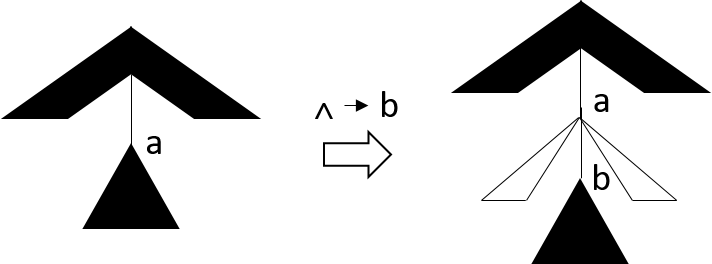
\includegraphics[width=0.4\linewidth]{Insertion}
	\label{Insertion} 
	\centering
\end{figure}
\item \textbf{Deletion.} deletion of a node
\begin{figure}
	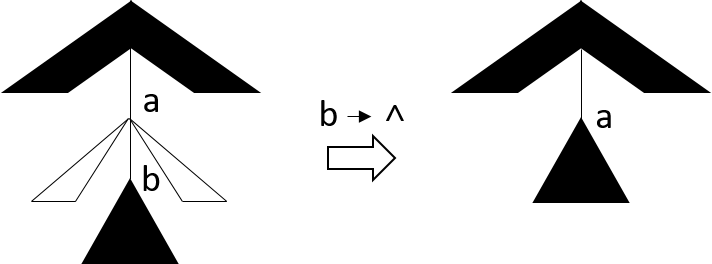
\includegraphics[width=0.4\linewidth]{Delete}
	\label{Deletion} 
	\centering
\end{figure}
\item \textbf{Substitution.} replace a label of a node by another label. This operation does not affect the skeleton of the tree.
\begin{figure}
	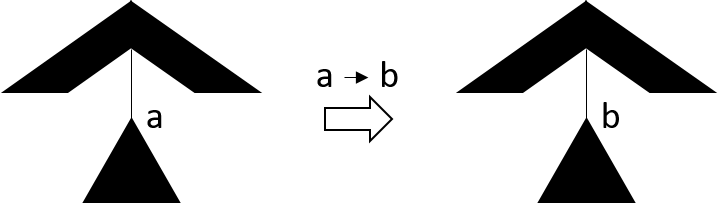
\includegraphics[width=0.4\linewidth]{Replacement}
	\label{Substitution} 
	\centering
\end{figure}
\end{itemize}
\end{itemize}
\end{frame}

%------------------------------------------------
\section{Notation}
\begin{frame}
\frametitle{Notation}
\begin{itemize}
\item \textbf{Tree} 
\begin{columns}[c] % The "c" option specifies centered vertical alignment while the "t" option is used for top vertical alignment
\column{.45\textwidth} % Left column and width
\begin{itemize}
\item $l(f)$
\begin{figure}
	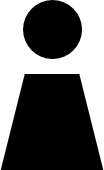
\includegraphics[width=0.2\linewidth]{Tree}
	\label{Tree} 
	\centering
\end{figure}
\end{itemize}
\column{.45\textwidth} % Left column and width
\begin{itemize}
\item $l(A_1 \comp A_2 \comp \cdots \comp A_n)$
\begin{figure}
	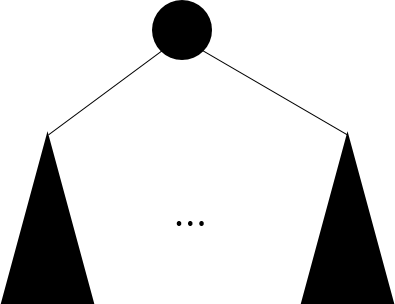
\includegraphics[width=0.5\linewidth]{Tree2}
	\label{Another Tree Representation} 
	\centering
\end{figure}
\end{itemize}
\end{columns}
\item \textbf{Forest} 
\begin{columns}[c] % The "c" option specifies centered vertical alignment while the "t" option is used for top vertical alignment
\column{.45\textwidth} % Left column and width
\begin{itemize}
\item $l(f) \comp t$
\begin{figure}
	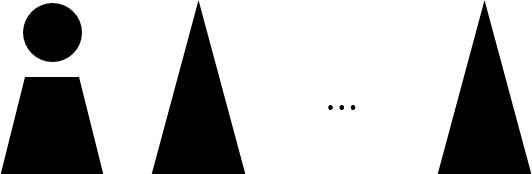
\includegraphics[width=0.8\linewidth]{Forest}
	\label{Forest} 
	\centering
\end{figure}
\end{itemize}
\column{.45\textwidth} % Left column and width
\begin{itemize}
\item $t \comp l(f)$
\begin{figure}
	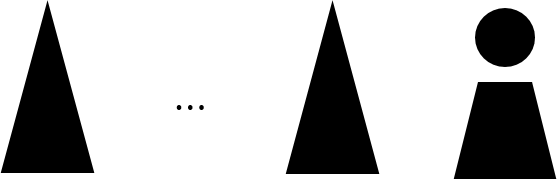
\includegraphics[width=0.8\linewidth]{Forest2}
	\label{Another Forest Representation} 
	\centering
\end{figure}
\end{itemize}
\end{columns}
\end{itemize}
\end{frame}

%------------------------------------------------

\begin{frame}
\frametitle{Notation}
\begin{columns}[c]
\column{.3\textwidth}
\begin{itemize}
\item \emph{$\left\vert F \right\vert$} 
\item \emph{$\#leaves(F)$} 
\item \emph{$height(F)$} 
\item \emph{$F(i)$} 
\item \emph{$root(F)$}
\item \emph{$F(i)^{\comp}$}
\item \emph{$\#deg(i)$} 
\item \emph{$\#anc(i)$} 
\end{itemize}
\column{.7\textwidth}
\begin{itemize}[]
\item[]  the number of nodes of the forest F.
\item[]  the number of leaves of F.
\item[]  the maximal height of the tress composing F.
\item[]  the subtree of F rooted at node i.
\item[]  the root of F.
\item[] $F(i) - root(F(i))$
\item[]  the number of direct children of node i.
\item[]  the number of ancestors of node i. 
\end{itemize}
\end{columns}

\textbf{Note:} 
\begin{itemize}
\item each node is its own ancestor.
\item  node j is a \textbf{proper ancestor} of node i if the path length from j to i is not 0.
\end{itemize}
\end{frame}

%------------------------------------------------
\section{A Simple Algorithm}
\subsection{Key Idea}
\begin{frame}
\frametitle{Key Idea(Naive Algorithm)}
\textbf{LEMMA 1}

Let $F_1(l(f) \comp t)$ and $F_2(l'(f') \comp t')$ be \textbf{ordered forest} and $\gamma$ be a metric cost function defined on labels. We have the forest distance $\delta(F_1, F_2)$
\begin{flalign}
&\delta(\theta, \theta) = 0 &\\
&\delta(l(f) \comp t, \theta) = \delta(f \comp t, \theta) + \gamma(l \to \lambda) &\\
&\delta(\theta, l'(f') \comp t') = \delta(\theta, f' \comp t') + \gamma(\lambda \to l') &\\
&\delta(l(f) \comp t, l'(f') \comp t') = min \begin{cases}
	  \delta(f \comp t, l'(f') \comp t') + \gamma(l \to \lambda) \\ %& \text{deletion of l,}\\
      \delta(l(f) \comp t, f' \comp t') + \gamma(\lambda \to l') \\ %& \text{insertion of l',}\\
     \delta(f, f') + \delta(t, t') + \gamma(l \to l') & \\ %\text{replacement of l by l'}
      \end{cases} &
\end{flalign}

\end{frame}

%------------------------------------------------
\subsection{Time Complexity}
\begin{frame}
\frametitle{Time Complexity(Naive Algorithm)}
\begin{block}{Prerequisite of the Analysis}
\begin{itemize}
\item Lemma 1 implies dynamic programming.
\item Each new subproblem can be computed in constant time.
\item Time complexity is bounded by $\#subproblems\ of\ F_1 * \#subproblems\ of\ F_2$. 
\end{itemize}
\end{block}
\begin{block}{Count the subproblems of F}
\begin{itemize}
\item  $\#subproblem\ of\ F = \#(i,j)-deleted\ subforest$, $0 \leq i + j \leq \left\vert F \right\vert$ 
\item $\#(i, j)-deleted\ subforest = \sum_{k=0}^{\left\vert F \right\vert}k = \mathcal{O}(\left\vert F \right\vert^2)$, since for each i there are $\left\vert F \right\vert - i$ choices for j
\item numerous redundant subforests.
\end{itemize}
\end{block}
\begin{block}{Conclusion}
Time complexity is bounded by $\mathcal{O}(\left\vert F_1 \right\vert^2 \left\vert F_2 \right\vert^2)$. 
\end{block}
\end{frame}
%------------------------------------------------
\section{Zhang and Shasha's algorithm}
\subsection{Key Idea}
\begin{frame}
\frametitle{Key Idea(Zhang and Shasha's Algorithm)}
\textbf{LEMMA 2}
\begin{block}{For tree-tree edit distance}
\begin{flalign}
&\delta(l(f), l'(f')) = min \begin{cases}
	  \delta(f , l'(f')) + \gamma(l \to \lambda) \\ %& \text{deletion of l,}\\
      \delta(l(f), f') + \gamma(\lambda \to l') \\ %& \text{insertion of l',}\\
     \delta(f, f') + \gamma(l \to l') & \\ %\text{replacement of l by l'}
      \end{cases} &
\end{flalign}
\end{block}
\begin{block}{For forest-forest edit distance}
\begin{flalign}
&\delta(l(f) \comp t, l'(f') \comp t') = min \begin{cases}
	  \delta(f \comp t , l'(f') \comp t') + \gamma(l \to \lambda) \\ %& \text{deletion of l,}\\
      \delta(l(f) \comp t, f' \comp t') + \gamma(\lambda \to l') \\ %& \text{insertion of l',}\\
     \delta(l(f), l'(f')) + \delta(t, t') & \\ %\text{replacement of l by l'}
      \end{cases} &
\end{flalign}
\end{block}
\end{frame}

%------------------------------------------------
\begin{frame}
\frametitle{Key Idea(Zhang and Shasha's Algorithm)}
The lemma 2 is correct.

\emph{Proof.}

For tree-tree distance, formula 
\begin{displaymath}
\delta(l(f), l'(f')) \leq \delta(f, f') + \gamma(l, l')
\end{displaymath}
represents a particular mapping of $\delta(l(f), l'(f'))$
\begin{figure}
	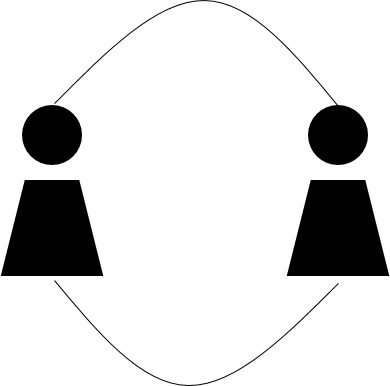
\includegraphics[width=0.3\linewidth]{treetree}
	\label{Tree-Tree Distance} 
	\centering
\end{figure}
\end{frame}

%------------------------------------------------
\begin{frame}
\frametitle{Key Idea(Zhang and Shasha's Algorithm)}
The lemma 2 is correct.

\emph{Proof.Continue}

For forest-forest distance, formula 
\begin{displaymath}
\delta(l(f) \comp t, l'(f') \comp t') \leq \delta(l(f), l'(f')) + \delta(t, t')
\end{displaymath}
represents a particular mapping of $\delta(l(f) \comp t, l'(f') \comp t')$
\begin{figure}
	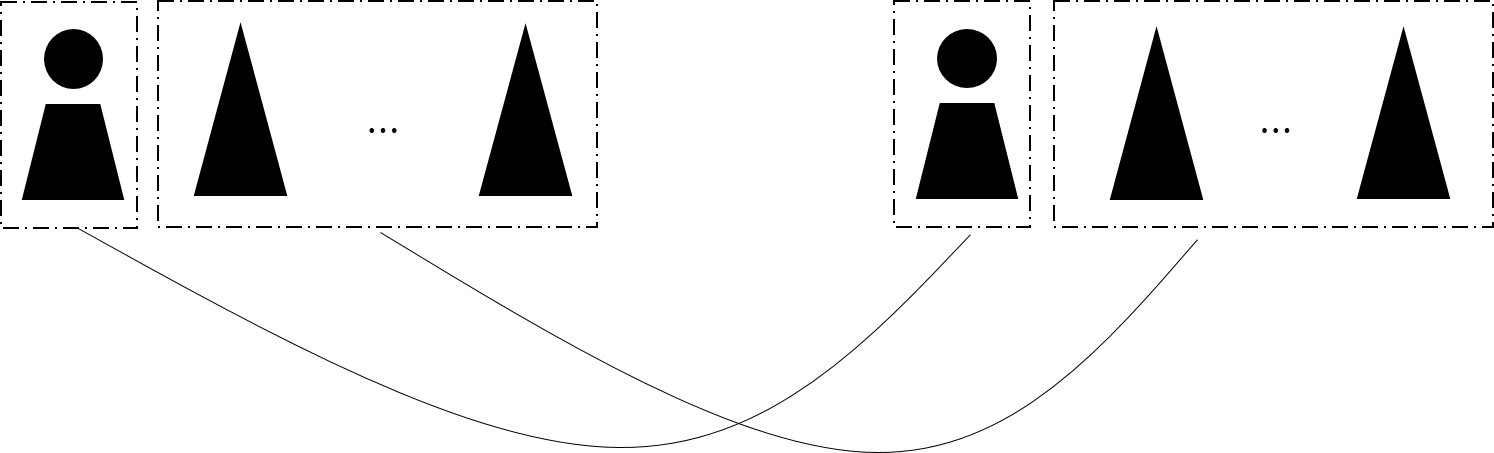
\includegraphics[width=0.8\linewidth]{forestforest}
	\label{Forest-Forest Distance} 
	\centering
\end{figure}
\end{frame}

%------------------------------------------------
\begin{frame}
\frametitle{Key Idea(Zhang and Shasha's Algorithm)}
The lemma 2 is correct.

\emph{Another Proof.}

Naive Algorithm
\begin{displaymath}
\delta(l(f) \comp t, l'(f') \comp t') = min \begin{cases}
	  \delta(f \comp t, l'(f') \comp t') + \gamma(l \to \lambda) \\ %& \text{deletion of l,}\\
      \delta(l(f) \comp t, f' \comp t') + \gamma(\lambda \to l') \\ %& \text{insertion of l',}\\
     \delta(f, f') + \delta(t, t') + \gamma(l \to l') & \\ %\text{replacement of l by l'}
      \end{cases}
\end{displaymath}
Zhang-Shasha's Algorithm
\begin{displaymath}
\delta(l(f) \comp t, l'(f') \comp t') = min \begin{cases}
	  \delta(f \comp t, l'(f') \comp t') + \gamma(l \to \lambda) \\ %& \text{deletion of l,}\\
      \delta(l(f) \comp t, f' \comp t') + \gamma(\lambda \to l') \\ %& \text{insertion of l',}\\
     \delta(l(f), l'(f')) + \delta(t, t')& \\ %\text{replacement of l by l'}
      \end{cases}
\end{displaymath}
\end{frame}

%------------------------------------------------
\begin{frame}
\frametitle{Key Idea(Zhang and Shasha's Algorithm)}
\begin{itemize}
\item dynamic programming style algorithm
\item bottom-up procedure
\item compute tree-tree distance between subtrees rooted at keyroots of both tree to avoid redundant computation.
\begin{figure}
	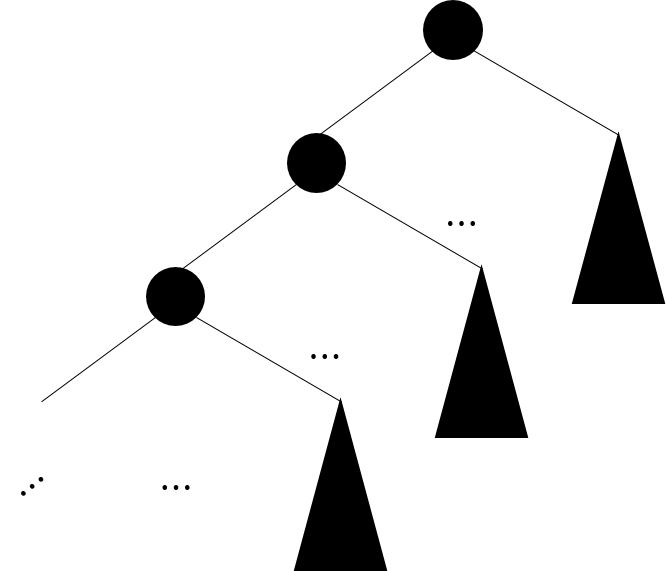
\includegraphics[width=0.5\linewidth]{bottomup}
	\label{Implications} 
	\centering
\end{figure}
\end{itemize}
\end{frame}


%------------------------------------------------
\subsection{Key Concept}
\begin{frame}
\frametitle{Key Concept(Zhang and Shasha's Algorithm)}
We define keyroot of T as
\begin{displaymath}
keyroots(T)\ =\ \{k\ |\ k\ is\ either\ root(T)\ or\ k\ has\ at\ least\ one\ siblings\}.
\end{displaymath} 
\begin{figure}
	\centering  
		{  
			\subfigure[] {\includegraphics[width=3cm,clip]{tree3}  }  
			\subfigure[] {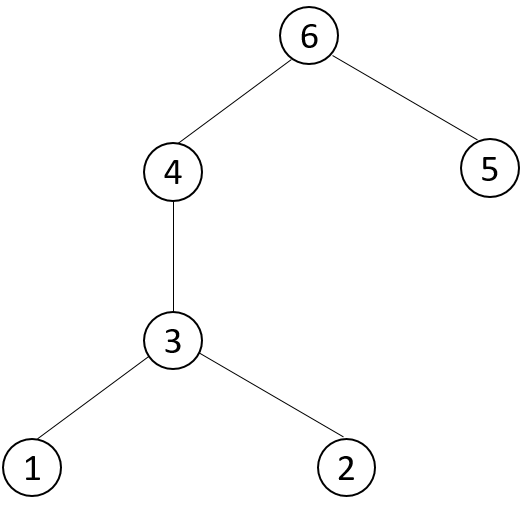
\includegraphics[width=3cm,clip]{tree4}  } 
		}
		\caption{compute the edit distance between tree(a) and tree(b)}
\end{figure}
keyroot($T_1$) = \{3, 5, 6\}

keyroot($T_2$) = \{2, 5, 6\}
\end{frame}


%------------------------------------------------
\subsection{Time Complexity}
\begin{frame}
\frametitle{Time Complexity(Zhang and Shasha's Algorithm)}
\begin{block}{Prerequisite of the Analysis}
\begin{itemize}
\item The time complexity is bounded by 
\begin{displaymath}
\sum_{i=1}^{i=\left\vert keyroots(T_1) \right\vert} \left\vert T_1(keyroots(T_1)[i]) \right\vert * \sum_{i=1}^{i=\left\vert keyroots(T_2) \right\vert} \left\vert T_2(keyroots(T_2)[i]) \right\vert
\end{displaymath}
\end{itemize}
\end{block}
\end{frame}

%------------------------------------------------
\begin{frame}
\frametitle{Time Complexity(Zhang and Shasha's Algorithm)}
\begin{block}{Prerequisite of the Analysis}
\begin{itemize}
\item Define for each node i, 
\begin{displaymath}
cdepth(i) = \left\vert anc(i) \cap keyroots(T) \right\vert
\end{displaymath}
Define for a tree T, 
\begin{displaymath}
cdepth(T) = max\ cdepth(i)
\end{displaymath}
\item \textbf{Lemma 3} 
\begin{displaymath}
\left\vert keyroot(T) \right\vert \leq \left\vert leaves(T) \right\vert
\end{displaymath}, since each leaf is the leftmost descendant of at most one member of keyroot(T).
\item From definition and Lemma 3 $cdepth(i) \leq min(depth(T), leaves(T))$ for $1 \leq i \leq \left\vert T \right\vert$. Hence, $cdepth(T) \leq min(depth(T), leaves(T))$.
\end{itemize}
\end{block}
\end{frame}

%------------------------------------------------
\begin{frame}
\frametitle{Time Complexity(Zhang and Shasha's Algorithm)}
\begin{block}{Prerequisite of the Analysis}
\begin{itemize}
\item \textbf{Lemma 4} 
\begin{displaymath}
\sum_{i=1}^{i=\left\vert keyroots(T) \right\vert} \left\vert T(keyroots(T)[i]) \right\vert = \sum_{j=1}^{j=\left\vert T \right\vert}cdepth(j)
\end{displaymath}, each node j is counted cdepth(j) times.
\end{itemize}
\end{block}
\end{frame}

%------------------------------------------------
\begin{frame}
\frametitle{Time Complexity(Zhang and Shasha's Algorithm)}
\begin{block}{Conclusion}
\begin{itemize}
\item Time Complexity
\begin{eqnarray*}
\begin{split}
& \sum_{i=1}^{i=\left\vert keyroots(T_1) \right\vert}\sum_{j=1}^{j=\left\vert keyroots(T_2) \right\vert}T_1(keyroots(T_1)[i]) * T_2(keyroots(T_2)[j])\\
& =\sum_{i=1}^{i=\left\vert T_1 \right\vert}cdepth(i) * \sum_{j=1}^{j=\left\vert T_2 \right\vert}cdepth(j)\\ 
& \leq \left\vert T_1 \right\vert * cdepth(T_1) * \left\vert T_2 \right\vert * cdepth(T_2)\\
\end{split}
\end{eqnarray*}
\item Hence we can conclude that the time complexity is 
\begin{displaymath}
\mathcal{O}(\left\vert T_1 \right\vert * \left\vert T_2 \right\vert * min(depth(T_1), leaves(T_1)) * min(depth(T_2), leaves(T_2)))
\end{displaymath}
\end{itemize}
\end{block}
\end{frame}

%------------------------------------------------
\section{Klein's Algorithm}
\subsection{Definition}
\begin{frame}
\frametitle{Definition(Klein's Algorithm)}
\begin{block}{Leftmost decomposition}
\begin{displaymath}
\delta(t \comp l(f), t' \comp l'(f')) = min \begin{cases}
		\gamma(l \to \lambda) + \delta(t \comp f, t' \comp l'(f'))  \\%&\text{deletion of l}\\
        \gamma(\lambda \to l') + \delta(t \comp l(f), t' \comp f') \\%&\text{insertion of l'}\\
        \delta(l(f), l'(f')) + \delta(t, t') %&\text{replacement of l by l'}								
								\end{cases}
\end{displaymath}
\end{block}
\begin{block}{Rightmost decomposition}
\begin{displaymath}
\delta(l(f) \comp t, l'(f') \comp t') = min \begin{cases}
		\gamma(l \to \lambda) + \delta(f \comp t, l'(f') \comp t')  \\%&\text{deletion of l}\\
        \gamma(\lambda \to l') + \delta(l(f) \comp t, f' \comp t') \\%&\text{insertion of l'}\\
        \delta(l(f), l'(f')) + \delta(t, t') %&\text{replacement of l by l'}								
								\end{cases}
\end{displaymath}
\end{block}
\end{frame}

%------------------------------------------------
\subsection{Observation}
\begin{frame}
\frametitle{Observation(Klein's Algorithm)}
Left Decomposition
\begin{figure}
	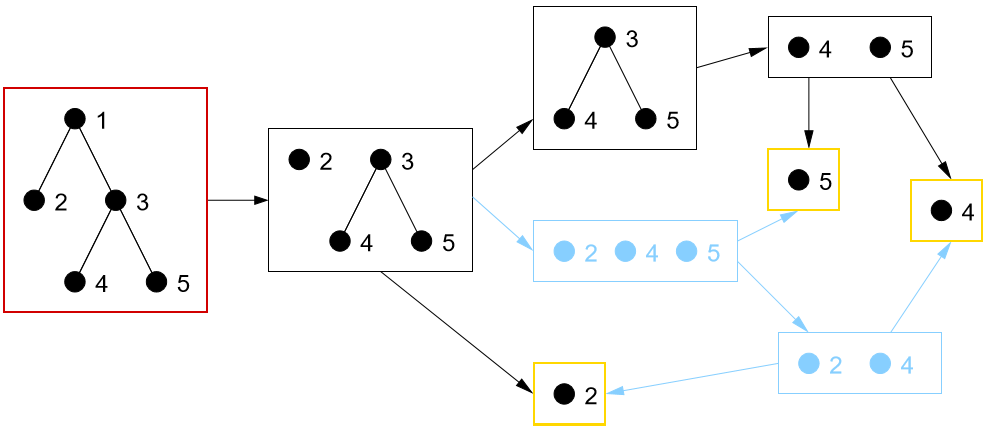
\includegraphics[width=0.48\linewidth]{leftdecomposition}
	\label{Left Decomposition} 
	\centering
\end{figure}
gives 7 sub-forests.

Right Decomposition
\begin{figure}
	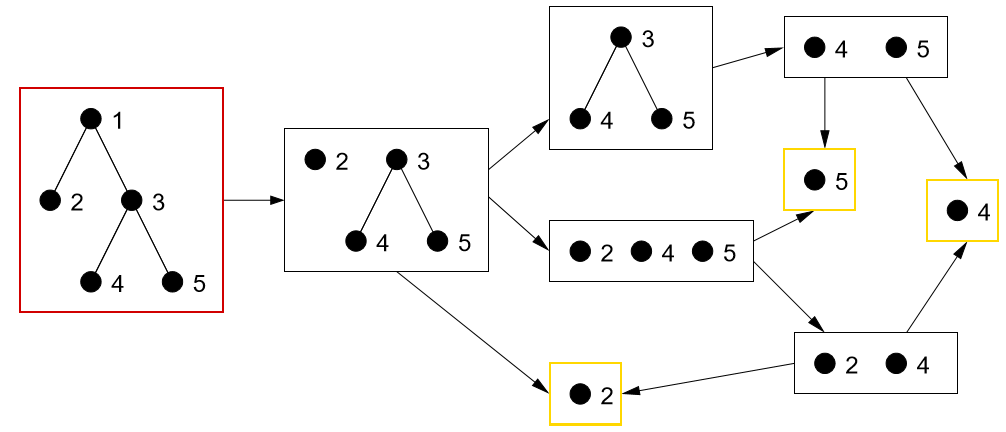
\includegraphics[width=0.48\linewidth]{rightdecomposition}
	\label{right Decomposition} 
	\centering
\end{figure}
gives 9 sub-forests.
\end{frame}

%------------------------------------------------
\subsection{Key Idea}
\begin{frame}
\frametitle{Key Idea(Klein's Algorithm)}
\begin{itemize}
\item Optimize the subproblems of a forest$(l(f) \comp t)$ by eliminating nodes of $f$ in $f \comp t$, so that $f \comp t$ and $t$ share relevant forests as most as possible.
\item However, this method also loses the ability to control the second forest$(l'(f') \comp t')$
\end{itemize}
\begin{figure}
	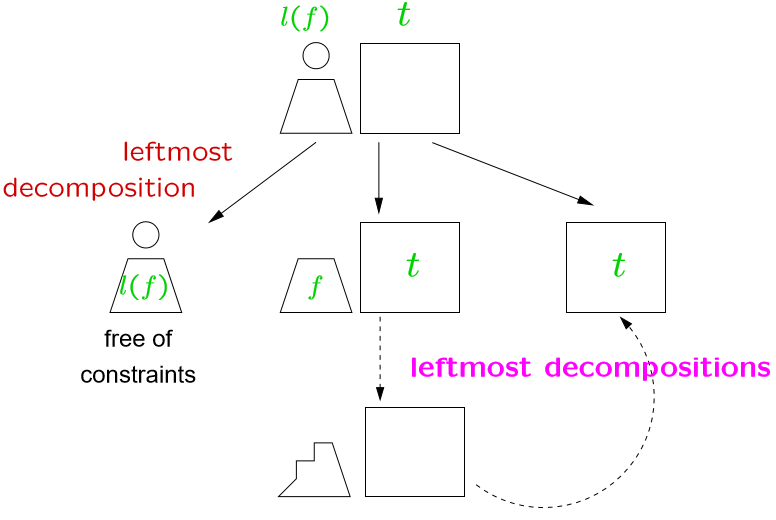
\includegraphics[width=0.6\linewidth]{economicalstrategy}
	\label{Economical Strategy} 
	\centering
\end{figure}
\end{frame}

%------------------------------------------------
\subsection{Key Concept}
\begin{frame}
\frametitle{Key Concept(Klein's Algorithm)}
\begin{itemize}
\item \textbf{heavy child.} $heavy(i)$ denote the child of i having greatest weight.
\item \textbf{heavy path.} The sequence of nodes $i, heavy(i), heavy(heavy(i)), \cdots$ defines a descending path which is called the heavy path.
\end{itemize}
\begin{figure}
	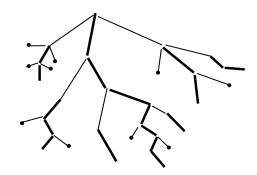
\includegraphics[width=0.4\linewidth]{heavypath}
	\label{Heavy Path}
	\centering
\end{figure}
\end{frame}

%------------------------------------------------
\subsection{Algorithm}
\begin{frame}
\frametitle{Algorithm(Klein's Algorithm)}
uses the heavy path as a guide for the decomposition of the forest.

Let $l(f) \comp t$ be the forest to be decomposed.
compute the heavy path P for $l(f) \comp t$

\begin{enumerate}[1)]
\item if $l$ belongs to P, apply $t \comp l(f)$. Otherwise, apply $l(f) \comp t$.
\item apply this scheme recursively to all sub-forests of $l(f) \comp t$.
\end{enumerate}

\begin{figure}
	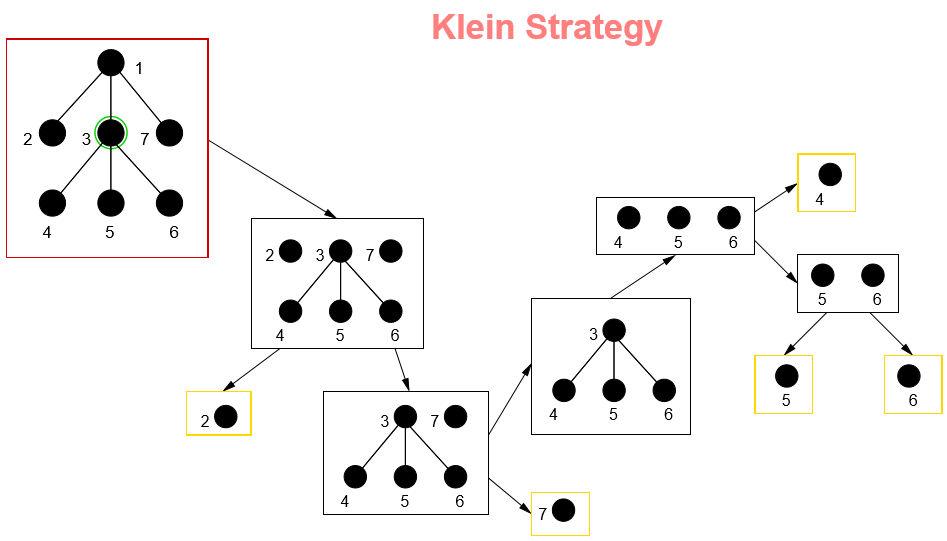
\includegraphics[width=0.7\linewidth]{heavypathdecomposition}
	\label{Heavy Path Decomposition} 
	\centering
\end{figure}
\end{frame}

%------------------------------------------------
\subsection{Time Complexity}
\begin{frame}
\frametitle{Time Complexity(Klein's Algorithm)}
\begin{block}{Prerequisite of the Analysis}
\begin{itemize}
\item Define one of node i 's children with maximal number of descendants and marks it as \emph{heavy}, and we mark all the other children of i as \emph{light}
\item The time complexity is bounded by 
\begin{displaymath}
\sum_{i \in light(T_1)} \left\vert T_1(i) \right\vert * \left\vert T_2 \right\vert^2
\end{displaymath}
\end{itemize}
\end{block}
\end{frame}
%------------------------------------------------
\begin{frame}
\frametitle{Time Complexity(Klein's Algorithm)}
\begin{block}{Prerequisite of the Analysis}
\begin{itemize}
\item Define ldepth(i) to be the number of light nodes that are \textbf{proper ancestors} of i in F. 
\item \textbf{Theorem 1}(Sleator and Tarjan, 1983)

Let v be any vertex of tree F. There is at most one heavy edge entering v, and there are at most $log_2 \left\vert F \right\vert$ light edges on the tree path from v to root(v).

\item According to theorem 1, for each node i in tree F, we have 
\begin{displaymath}
ldepth(i) \leq log_2 \left\vert F \right\vert
\end{displaymath}

\end{itemize}
\end{block}
\end{frame}

%------------------------------------------------
\begin{frame}
\frametitle{Time Complexity(Klein's Algorithm)}
\begin{block}{Conclusion}
\begin{itemize}
\item Subforests of $T_1$
\begin{eqnarray*}
\begin{split}
& \sum_{i \in light(T_1)} \left\vert T_1(i) \right\vert\\
& \leq \sum_{i \in T_1}(1 + ldepth(i))\\ 
& \leq \sum_{i \in T_1}(log_2\left\vert T_1 \right\vert + \mathcal{O}(1))\\
& = \mathcal{O}(\left\vert T_1 \right\vert log_2\left\vert T_1\right\vert)
\end{split}
\end{eqnarray*}
\item Hence the time complexity is $\mathcal{O}(\left\vert T_1 \right\vert log_2\left\vert T_1\right\vert * \left\vert T_2 \right\vert^2)$
\end{itemize}
\end{block}
\end{frame}
%------------------------------------------------
\section{Decomposition Strategies}
\begin{frame}
\frametitle{Decomposition Strategies}
\textbf{Lemma 5}
\begin{itemize}
\item if F or F' is an empty forest:

$R(\epsilon , l(f) \comp t) = {(\epsilon, l(f) \comp t)} \cup R(\epsilon, f \comp t)\ whenever\ \phi(\epsilon, l(f) \comp t) = left,$

$R(\epsilon, t \comp l(f)) = {(\epsilon, t \comp l(f))} \cup R(\epsilon, t \comp f)\ whenever\ \phi(\epsilon, t \comp l(f)) = right,$

$R(l(f) \comp t, \epsilon ) = {(l(f) \comp t, \epsilon)} \cup R(f \comp t, \epsilon)\ whenever\ \phi(l(f) \comp t, \epsilon) = left,$

$R(t \comp l(f), \epsilon) = {(t \comp l(f), \epsilon)} \cup R(t \comp f, \epsilon)\ whenever\ \phi(t \comp l(f), \epsilon) = right,$

\item $if\ (F, F') = (l(f) \comp t, l'(f') \comp t')\ and\ \phi(F, F') = left,\ then$

$R(F, F') = {(F, F')} \cup R(f \comp t, F') \cup R(F, f' \comp t') \cup R(l(f), l'(f')) \cup R(t, t')$

\item $if\ (F, F') = (t \comp l(f), t' \comp l'(f'))\ and\ \phi(F, F') = right,\ then$

$R(F, F') = {(F, F')} \cup R(t \comp f, F') \cup R(F, t \comp f) \cup R(l(f), l'(f')) \cup R(t, t')$
\end{itemize}
\end{frame}

%------------------------------------------------
\begin{frame}
\frametitle{Lower Bound of Relevant Forests}
\textbf{Lemma 6}
\begin{itemize}
\item $R(l(f)) = \{l(f)\} \cup R(f)$, no matter what the direction is. 

That is to say, $\#ref(l(f)) \geq \left\vert l(f) \right\vert $ 
\item $R(l(f) \comp t) = \{(l(f) \comp t)\} \cup R(f \comp t) \cup R(l(f)) \cup R(t)$, if the direction is left. 

That is to say, $\#ref(l(f) \comp t) \geq \#ref(l(f)) + \#ref(t)$
\item $R(t \comp l(f)) = \{(t \comp l(f))\} \cup R(t \comp f) \cup R(l(f)) \cup R(t)$, if the direction is right.
\end{itemize}
\end{frame}

%------------------------------------------------
\begin{frame}
\frametitle{Lower Bound of Relevant Forests}
\textbf{Lemma 7}

Given a tree A=$l(A_1 \comp A_2 \comp \cdots \comp A_n)$, for any strategy we have,

$\#rel(A) \geq \left\vert A \right\vert - \left\vert A_i \right\vert + \#rel(A_1) + \cdots + \#rel(A_n)$

, where i $\in$ [1 $\cdots$ n] is such that size of $A_i$ is maximal.
\begin{figure}
	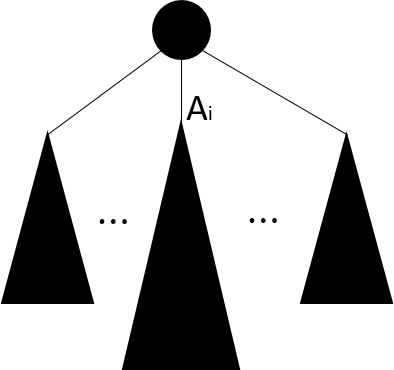
\includegraphics[width=0.3\linewidth]{lemma7}
	\label{Lemma 7} 
	\centering
\end{figure}
\end{frame}

%------------------------------------------------
\begin{frame}
\frametitle{Lower Bound of Relevant Forests}
\textbf{Lemma 7}

Given a tree A=$l(A_1 \comp A_2 \comp \cdots \comp A_n)$, for any strategy we have,

$\#rel(A) \geq \left\vert A \right\vert - \left\vert A_i \right\vert + \#rel(A_1) + \cdots + \#rel(A_n)$

, where i $\in$ [1 $\cdots$ n] is such that size of $A_i$ is maximal.

\vspace{12pt} 
\emph{Proof.}

From lemma 6, $R(l(f)) = {l(f)} \cup R(f)$. That is to say, 

$\#rel(l(f)) = 1 + \#rel(f)$.

\vspace{6pt} 
Then let $F=A_1 \comp \cdots \comp A_n$. To prove lemma 7, we first prove that 

$\#ref(F) \geq \left\vert F \right\vert - \left\vert A_i \right\vert + \#ref(A_1) + \cdots + \#ref(A_n)$
\end{frame}

%------------------------------------------------
\begin{frame}
\frametitle{Lower Bound of Relevant Forests}
\textbf{Lemma 7}

Given a tree A=$l(A_1 \comp A_2 \comp \cdots \comp A_n)$, for any strategy we have,

$\#rel(A) \geq \left\vert A \right\vert - \left\vert A_i \right\vert + \#rel(A_1) + \cdots + \#rel(A_n)$

, where i $\in$ [1 $\cdots$ n] is such that size of $A_i$ is maximal.

\vspace{12pt} 
\emph{Proof.}

For case n = 1, $\#ref(A_1) \geq \left\vert A_1 \right\vert - \left\vert A_1 \right\vert + \#ref(A_1)$

\vspace{6pt} 
For case $n > 1$, let \textbf{$F = l(g) \comp A_2 \cdots A_n$}, \textbf{t be $A_2 \comp \cdots \comp A_n$} then by lemma 5,

$R(F) = \{F\} \cup R(g \comp t) \cup R(A_1) \cup R(t)$

From lemma 6, we know,

$R(g \comp t) \geq \left\vert g \right\vert + \left\vert t \right\vert \geq min\{\left\vert g \right\vert, \left\vert t \right\vert \}$

By applying the inequality, we have    

$\#ref(F) \geq 1 + \#ref(A_1) + \#ref(t) + min\{\left\vert g \right\vert, \left\vert t \right\vert \}$
\end{frame}

%------------------------------------------------
\begin{frame}
\frametitle{Lower Bound of Relevant Forests}
\textbf{Lemma 7}

Given a tree A=$l(A_1 \comp A_2 \comp \cdots \comp A_n)$, for any strategy we have,

$\#rel(A) \geq \left\vert A \right\vert - \left\vert A_i \right\vert + \#rel(A_1) + \cdots + \#rel(A_n)$

, where i $\in$ [1 $\cdots$ n] is such that size of $A_i$ is maximal.

\vspace{12pt} 
\emph{Proof.}

Applying induction hypothesis for $t=A_2 \comp \cdots \comp A_n$

$\#ref(F) \geq 1 + \#ref(A_1) + \cdots + \#ref(t) + \left\vert t \right\vert - \left\vert A_j \right\vert + min\{\left\vert g \right\vert, \left\vert t \right\vert \}$

\vspace{6pt} 
Then we need to prove that, $1 + \left\vert t \right\vert - \left\vert A_j \right\vert + min\{\left\vert g \right\vert, \left\vert t \right\vert\} \geq \left\vert F \right\vert - \left\vert A_i \right\vert$, where $A_i$ is the size of the largest sub-tree in forest $A_1 \comp \cdots \comp A_n$, while $A_j$ is the size of the largest sub-tree in forest $A_2 \comp \cdots \comp A_n$ 
\end{frame}

%------------------------------------------------
\begin{frame}
\frametitle{Lower Bound of Relevant Forests}
\textbf{Lemma 7}

Given a tree A=$l(A_1 \comp A_2 \comp \cdots \comp A_n)$, for any strategy we have,

$\#rel(A) \geq \left\vert A \right\vert - \left\vert A_i \right\vert + \#rel(A_1) + \cdots + \#rel(A_n)$

, where i $\in$ [1 $\cdots$ n] is such that size of $A_i$ is maximal.

\vspace{12pt} 
\emph{Proof.}

In the case when $\left\vert g \right\vert \leq \left\vert t \right\vert$, then we have $1 + \left\vert t\right\vert + \left\vert g\right\vert = \left\vert F \right\vert$. Since $\left\vert A_j \right\vert \leq \left\vert A_i \right\vert$, it follows that  $1 + \left\vert t \right\vert - \left\vert A_j \right\vert + min\{\left\vert g \right\vert, \left\vert t \right\vert\} \geq \left\vert F \right\vert - \left\vert A_i \right\vert$

\vspace{6pt} 
In the case when $\left\vert g \right\vert > \left\vert t \right\vert$, this implies that $A_1$ is the largest subtree of A. So $i = 1$ and $\left\vert F \right\vert -\left\vert A_i\right\vert = \left\vert t \right\vert$, that proves $1 + \left\vert t \right\vert - \left\vert A_j \right\vert + min\{\left\vert g \right\vert, \left\vert t \right\vert\} \geq \left\vert F \right\vert - \left\vert A_i \right\vert$

\end{frame}

%------------------------------------------------
\begin{frame}
\frametitle{Lower Bound of Relevant Forests}
\textbf{Lemma 7}

Given a tree A=$l(A_1 \comp A_2 \comp \cdots \comp A_n)$, for any strategy we have,

$\#rel(A) \geq \left\vert A \right\vert - \left\vert A_i \right\vert + \#rel(A_1) + \cdots + \#rel(A_n)$

, where i $\in$ [1 $\cdots$ n] is such that size of $A_i$ is maximal.

\vspace{12pt} 
\emph{Proof.}

To sum up, the number of relevant sub-forest of a tree A is 
\begin{eqnarray*}
\begin{split}
&\#ref(A) = 1 + \#rel(F) \\
& \ \ \ \ \ \ \ \ \ \ \ \ \geq 1 + \left\vert F \right\vert - \left\vert A_i \right\vert +\#rel(A_1) + \cdots + \#rel(A_n) \\
& \ \ \ \ \ \ \ \ \ \ \ \ = \left\vert A \right\vert - \left\vert A_i \right\vert + \#rel(A_1) + \cdots + \#rel(A_n) \\
\end{split}
\end{eqnarray*}
\end{frame}

%------------------------------------------------
\begin{frame}
\frametitle{Lower Bound of Relevant Forests}
\textbf{Lemma 8}
$\#rel(A)$ has a lower bound in $\mathcal{O}(nlog(n))$

\vspace{12pt} 
\emph{Proof.}
Let $T_n$ be a complete balanced binary tree of size n, we prove that $\#ref(T_n) \geq \frac{(n+1)log_2(n+1)}{2}$
\begin{figure}
	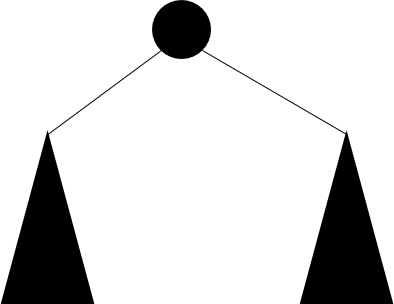
\includegraphics[width=0.3\linewidth]{completebinarytree}
	\label{Complete Binary Tree}
	\centering
\end{figure}

For case n = 1, $rel(T_n) = 1$, consistent with lemma 8.
\end{frame}

%------------------------------------------------
\begin{frame}
\frametitle{Lower Bound of Relevant Forests}
\textbf{Lemma 8}
$\#rel(A)$ has a lower bound in $\mathcal{O}(nlog(n))$

\vspace{12pt} 
\emph{Proof.}
Let $T_n$ be a complete balanced binary tree of size n, we prove that $\#ref(T_n) \geq \frac{(n+1)log_2(n+1)}{2}$

For case $n > 1$, by lemma 7, we have
\begin{displaymath}
\#rel(T_n) \geq n - m + 2 * \#ref(T_m)
\end{displaymath}
, where $m=(n-1)/2$. $T_n$ is of the form $l(A \comp B)$, where A and B are two complete balanced tree of size m.
By induction hypothesis for $T_m$, it converts to
\begin{eqnarray*}
\begin{split}
& \#ref(T_n) \geq n - m + (m + 1)log_2(m+1)\\
& \ \ \ \ \ \ \ \ \ \ \ \ \ =\frac{(n + 1)(log_2(m + 1) + 1)}{2}\\
& \ \ \ \ \ \ \ \ \ \ \ \ \ =\frac{(n + 1)(log_2(2m + 1) + 1)}{2}\\
& \ \ \ \ \ \ \ \ \ \ \ \ \ =\frac{(n+1)(log_2(n+1))}{2}\\
\end{split}
\end{eqnarray*}
\end{frame}

%------------------------------------------------
\begin{frame}
\frametitle{Lower Bound of Relevant Forests}
\textbf{Lemma 9}

Let A and B be two trees of size n. For any decomposition strategy, $\#rel(A, B)$ has a lower bound in $\mathcal{O}(n^2log^2(n))$
\end{frame}

%------------------------------------------------
\section{Cover Strategies}
\begin{frame}
\frametitle{Cover Strategies}
\begin{block}{Cover}
Let F be a tree, for each node i in F
\begin{itemize}
\item if $deg(i) = 0$ or $deg(i) = 1$, then $r(i) \in \{right, left\}$.
\item if $deg(i) > 1$, then r(i) is a favourite child of i.
\end{itemize}
\end{block}
\begin{block}{Cover Strategies}
\begin{itemize}
\item if $deg(i) = 0$ or $deg(i) = 1$, then $\phi(A(i), G) = r(i)$, for each forest G of B.
\item Otherwise,let A(i) is of the form $l(A_1 \comp \cdots A_p \comp \cdots \comp A_n)$
\begin{itemize}
\item $\phi(T \comp A_p \cdots \comp A_n, G) = left$, for each forest T of $A_1 \comp \cdots \comp A_{p-1}$
\item $\phi(A_p \comp T, G) = right$, for each forest T of $A_{p+1} \comp \cdots \comp A_n$
\end{itemize}
\end{itemize}
\end{block}
\begin{figure}
	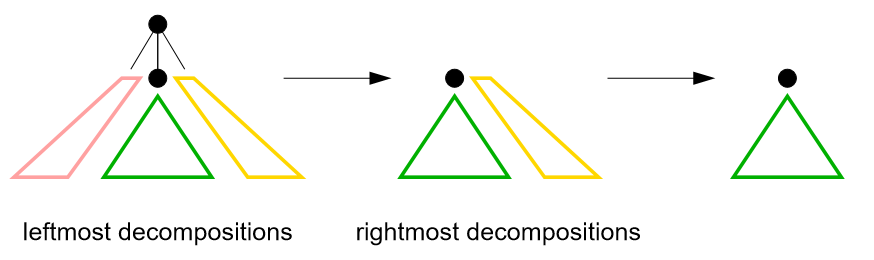
\includegraphics[width=0.55\linewidth]{favouritechild}
	\label{Favourite Child} 
	\centering
\end{figure}
\end{frame}
%------------------------------------------------
\begin{frame}
\frametitle{Cover Strategies}
\textbf{Zhang-Shasha Algorithms Cover Strategies}
\begin{itemize}
\item for any node of degree 0 or 1, the direction is right($t \comp l(f)$).
\item for any other node, the favorite child is the leftmost child. That is to say, the direction is right($t \comp l(f)$).
\end{itemize}

\textbf{Klein's Algorithm Cover Strategies}
\begin{itemize}
\item for any node of degree 0 or 1, the direction is left($l(f) \comp t$).
\item for any other node, the favorite child is the root of the heaviest subtree.
\end{itemize}

\begin{figure}
	\centering  
		{  
			\subfigure[] {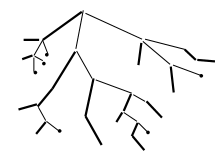
\includegraphics[width=4cm,clip]{zhangshasha}  }  
			\subfigure[] {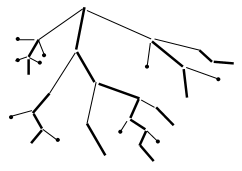
\includegraphics[width=4cm,clip]{klein}  } 
			
		}
	\caption{•}
\end{figure} 
\end{frame}


%------------------------------------------------
\begin{frame}
\frametitle{Exact Number of Relevant Forests}
\textbf{Lemma 10}

Let $A=l(A_1 \comp \cdots \comp A_n)$ be a cover tree such that $n=1$ or the root of $A_j$ is the favourite child.
\begin{displaymath}
\#rel(A) = \left\vert A \right\vert - \left\vert A_j \right\vert + \#rel(A_1) + \cdots + \#rel(A_n)
\end{displaymath}
\begin{figure}
	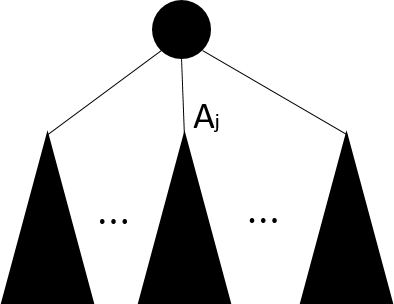
\includegraphics[width=0.3\linewidth]{lemma10}
	\label{LEMMA 10} 
	\centering
\end{figure}
\end{frame}

%------------------------------------------------

\begin{frame}
\frametitle{Upper Bound of Relevant Forests}
\textbf{Lemma 11}

Let $A=l(A_1 \comp \cdots \comp A_n)$ be a cover tree 
\begin{displaymath}
\#rel(A) \leq \frac{n(n+3)}{2} - \sum_{i \in A} \left\vert A(i) \right\vert
\end{displaymath}
In average
\begin{displaymath}
\frac{1}{2}n^2 + \frac{\sqrt{\pi}}{2}n^{\frac{3}{2}} +\mathcal{O}(n)
\end{displaymath}

\end{frame}

%------------------------------------------------
\begin{frame}
\frametitle{Happens of a Cover Strategy on a tree to Another Tree}
\textbf{Lemma 12}

Given a pair of tree (A, B) provided with a cover for A, all relevant forests of A fall within three categories:

\begin{itemize}
\item[$\alpha$] those that are compared with all rightmost forests of B,
\item[$\beta$] those that are compared with all leftmost forests of B,
\item[$\gamma$] those that are compared with all forests of B.
\end{itemize}

\begin{itemize}
\item $\#left(B)$ : number of leftmost subforests of B 
\item $\#right(B)$ : number of rightmost subforests of B
\item $\#speical(B)$ : number of all subforests of B
\end{itemize}

\textbf{Note:} $\#left(B)$, $\#right(B)$, $\#special(B)$ are known, depended by the structure of B
\end{frame}

%------------------------------------------------
\begin{frame}
\frametitle{Happens of a Cover Strategy on a tree to Another Tree}

\begin{itemize}
\item $\#left(B)$ : number of leftmost subforests of B 
\item $\#right(B)$ : number of rightmost subforests of B
\item $\#speical(B)$ : number of all subforests of B
\end{itemize}

\begin{figure}
	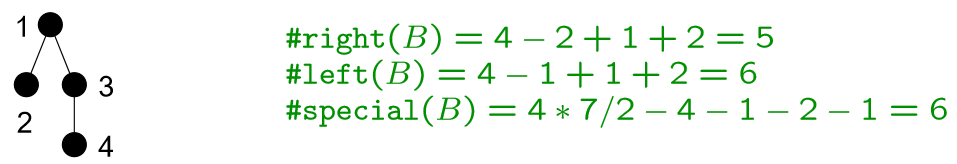
\includegraphics[width=1.0\linewidth]{exampleoflemma11}
	\label{Example of LEMMA 12} 
	\centering
\end{figure}

\end{frame}


%------------------------------------------------
\begin{frame}
\frametitle{Status of Nodes in a Cover Tree}

\begin{itemize}
\item \textbf{Free} : nodes that do not receive anything from the parent
\item \textbf{Left} :  nodes that inherit leftmost forests of B.
\begin{displaymath}
Left(A(i)) = (A(i), all\ leftmost\ forests\ of\ B)
\end{displaymath}
\item \textbf{Right} : nodes that inherit rightmost forests of B.
\begin{displaymath}
Right(A(i)) = (A(i), all\ rightmost\ forests\ of\ B)
\end{displaymath}
\item \textbf{All} : nodes that inherit all subforests of B from the parent
\begin{displaymath}
All(A(i)) = (A(i), all\ subforests\ of\ B)
\end{displaymath}
\end{itemize}

\textbf{Note1:}The status of a node depends of the direction and of the heritage from parent.

\textbf{Note2:}By definition, $\#rel(A, B)\ equals\ Free(A)$.
\end{frame}

%------------------------------------------------
\begin{frame}
\frametitle{Number of Relevant Forests of A Pair of Tree}
\textbf{LEMMA 13}

Let (A, B) be a pair of trees. A being a cover tree.

\begin{enumerate}[1)]
\item If A is reduced to a single node whose direction is right.
\begin{itemize}
\item Free(A) = Left(A) = $\#left(B)$
\item All(A) = Right(A) = $\#special(B)$
\end{itemize}
\item If A is reduced to a single node whose direction is left.
\begin{itemize}
\item Free(A) = Right(A) = \#right(B)
\item All(A) = Left(A) = \#special(B)
\end{itemize}
\end{enumerate}

\end{frame}


%------------------------------------------------
\begin{frame}
\frametitle{Number of Relevant Forests of A Pair of Tree}
\textbf{LEMMA 13}

Let (A, B) be a pair of trees. A being a cover tree.

\begin{enumerate}[1)]
\setcounter{enumi}{2}
\item If $A = l(A')$ and the direction of l is right
\begin{itemize}
\item Free(A) = Left(A) = $\#left(B) + Right(A')$

?? Free(A) = Left(A) = $\#left(B) + Left(A')$
\item All(A) = Right(A) = $\#special(B) + All(A')$
\end{itemize}
\item If $A = l(A')$ and the direction of l is left
\begin{itemize}
\item Free(A) = Right(A) = $\#right(B) + Left(A')$

?? Free(A) = Right(A) = $\#left(B) + Right(A')$
\item All(A) = Left(A) = $\#special(B) + All(A')$
\end{itemize}
\end{enumerate}


\begin{figure}
	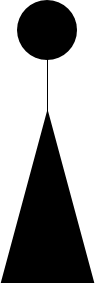
\includegraphics[width=0.08\linewidth]{lemma131}
	\label{LEMMA 13(1)} 
	\centering
\end{figure}
\end{frame}

%------------------------------------------------
\begin{frame}
\frametitle{Number of Relevant Forests of A Pair of Tree}
\textbf{LEMMA 13}

Let (A, B) be a pair of trees. A being a cover tree.

\begin{enumerate}[1)]
\setcounter{enumi}{4}
\item If $A=l(A_1 \comp \cdots \comp A_n)$ and the favourite child is $A_1$
\begin{itemize}
\item Free(A) = Left(A) = $\sum_{i>1}Free(A_i) + Left(A_1) + \#left(B)(\left\vert A \right\vert - \left\vert A_1 \right\vert)$
\item All(A) = Right(A) = $\sum_{i>1}Free(A_i) + All(A_1) + \#special(B)(\left\vert A \right\vert - \left\vert A_1 \right\vert)$
\end{itemize}
\item If $A=l(A_1 \comp \cdots \comp A_n)$ and the favourite child is $A_n$
\begin{itemize}
\item Free(A) = Left(A) = $\sum_{i<n}Free(A_i) + Left(A_n) + \#left(B)(\left\vert A \right\vert - \left\vert A_n \right\vert)$
\item All(A) = Right(A) = $\sum_{i<n}Free(A_i) + All(A_n) + \#special(B)(\left\vert A \right\vert - \left\vert A_n \right\vert)$
\end{itemize}
\end{enumerate}


\begin{figure}
	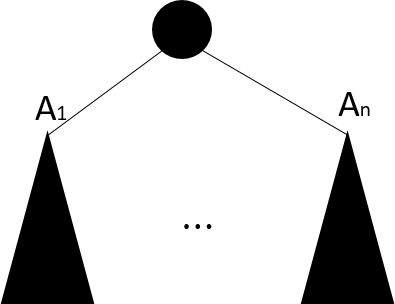
\includegraphics[width=0.4\linewidth]{lemma132}
	\label{LEMMA 13(2)} 
	\centering
\end{figure}
\end{frame}


%------------------------------------------------
\begin{frame}
\frametitle{Number of Relevant Forests of A Pair of Tree}
\textbf{LEMMA 13}

Let (A, B) be a pair of trees. A being a cover tree.

\begin{enumerate}[1)]
\setcounter{enumi}{6}
\item If $A=l(A_1 \comp \cdots \comp A_n)$ and the favourite child is $A_1$
\begin{itemize}
\item Free(A) = Right(A) = $\sum_{i\neq j}Free(A_i) + All(A_j) + \#right(B)(1 + \left\vert A_1 \comp \cdots \comp A_{j-1}\right\vert) + \#special(B)\left\vert A_{j+1} \comp \cdots \comp A_n\right\vert$
\item All(A) = Left(A) = $\sum_{i\neq j}Free(A_i) + All(A_j) + \#special(B)(\left\vert A \right\vert - \left\vert A_j \right\vert)$
\end{itemize}
\end{enumerate}


\begin{figure}
	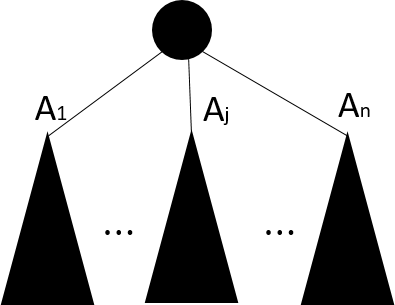
\includegraphics[width=0.4\linewidth]{lemma133}
	\label{LEMMA 13(3)} 
	\centering
\end{figure}
\end{frame}


%------------------------------------------------
\begin{frame}
\frametitle{Number of Relevant Forests of A Pair of Tree}
\textbf{Example of LEMMA 13}
\begin{figure}
	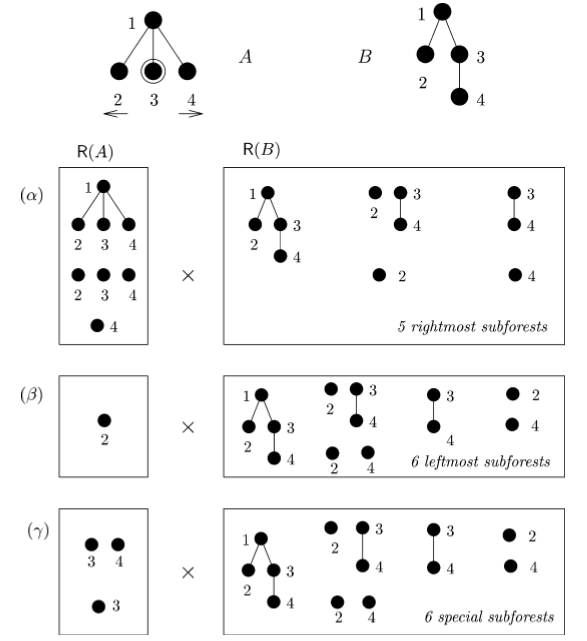
\includegraphics[width=0.5\linewidth]{exampleoflemma13}
	\label{Example of Lemma 13} 
	\centering
\end{figure}
gives 33 pairs of subforest.
\end{frame}

%------------------------------------------------
\begin{frame}
\frametitle{Number of Relevant Forests of A Pair of Tree}
\textbf{Example of LEMMA 13}
\begin{eqnarray*}
\begin{split}
& Free(A) = Free(2) + Free(4) + All(3) +\#special(B) * 1 + \#right(B) * 2\\
& \ \ \ \ \ \ \ \ \ \ =\#left(B) +\#right(B) +\#special(B) + \#special(B) \\
& \ \ \ \ \ \ \ \ \ \ \ \ \ + \#right(B) * 2\\
& \ \ \ \ \ \ \ \ \ \ =33
\end{split}
\end{eqnarray*}
\end{frame}

%------------------------------------------------

\begin{frame}
\frametitle{Number of Rightmost, Leftmost and Subforest.}
\textbf{LEMMA 14}

Let A be a tree,
\begin{displaymath}
\#right(A) = \sum(\left\vert A(i) \right\vert, i \in A) - \sum(\left\vert A(j) \right\vert, j\ is\ a\ rightmost\ child)
\end{displaymath}
\begin{displaymath}
\#left(A) = \sum(\left\vert A(i) \right\vert, i \in A) - \sum(\left\vert A(j) \right\vert, j\ is\ a\ leftmost\ child)
\end{displaymath}
\emph{Proof}.

From lemma 10, let A be $l(A_1 \comp \cdots \comp A_n)$, then 
\begin{displaymath}
\#right(A)=\sum_i\#right(A_i) + \left\vert A \right\vert - \left\vert A_n \right\vert
\end{displaymath}
\end{frame}

%------------------------------------------------

\begin{frame}
\frametitle{Number of Rightmost, Leftmost and Subforest.}
\textbf{LEMMA 15}

Let F be a forest of size n,
\begin{displaymath}
\#special(F) = \frac{n(n+3)}{2} - \sum_{i \in F} \left\vert F(i) \right\vert
\end{displaymath}

\emph{Proof}

For case $n = 0$, then $\#special(F)$ = 0, which is consistent with lemma 15.

\vspace{12pt} 
For case $n > 1$, let $F = l(g) \comp t$. There are two kinds of special sub-forest of F to be considered:
\begin{itemize}
\item those containing the node $l$: there are $\left\vert t \right\vert + 1$ such sub-forest
\item those not containing the node $l$:there are $\#special(g \comp t)0$ such sub-forest
\end{itemize}
\end{frame}


%------------------------------------------------

\begin{frame}
\frametitle{Number of Rightmost, Leftmost and Subforest.}
\textbf{LEMMA 15}

Let F be a forest of size n,
\begin{displaymath}
\#special(F) = \frac{n(n+3)}{2} - \sum_{i \in F} \left\vert F(i) \right\vert
\end{displaymath}

\emph{Proof}

This allows that 
\begin{displaymath}
\#special(F) = \left\vert t \right\vert + 1 + \#special(g \comp t)
\end{displaymath}
On one hand, $\left\vert t \right\vert + 1 = n - \left\vert l(g) \right\vert + 1$

On the other hand, by applying the hypothesis on $g \comp t$, whose size is n-1
\begin{displaymath}
\#special(g \comp t) = \frac{(n-1)(n+2)}{2} - \sum_{i \in g \comp t} \left\vert g \comp t(i) \right\vert
\end{displaymath}
Since $g\comp t$ is a sub-forest of F, this implies
\begin{displaymath}
\#special(g \comp t) = \frac{(n-1)(n+2)}{2} - \sum_{i \in g \comp t} \left\vert F(i) \right\vert
\end{displaymath}
\end{frame}

%------------------------------------------------

\begin{frame}
\frametitle{Number of Rightmost, Leftmost and Subforest.}
\textbf{LEMMA 15}

Let F be a forest of size n,
\begin{displaymath}
\#special(F) = \frac{n(n+3)}{2} - \sum_{i \in F} \left\vert F(i) \right\vert
\end{displaymath}

\emph{Proof}

It allows that 
\begin{eqnarray*}
\begin{split}
\#special(F) & = n - \left\vert l(g) \right\vert + 1 + \frac{(n-1)(n+2)}{2} - \sum_{i \in g \comp t}\left\vert F(i) \right\vert \\
& = n + 1 + \frac{(n-1)(n+2)}{2} - \sum_{i \in F} \left\vert F(i) \right\vert \\
& = \frac{n(n+3)}{2} - \sum_{i \in F}\left\vert F(i) \right\vert \\ 
\end{split}
\end{eqnarray*}
This concludes the proof.
\end{frame}

%------------------------------------------------

\begin{frame}
\frametitle{Number of Rightmost, Leftmost and Subforest.}
\textbf{LEMMA 16}

For Zhang and Shasha's algorithm, $\#rel(A, B) = \#left(A) * \#left(B)$.

\vspace{12pt} 
\emph{Proof}

Applying lemma 13, case 1, 3, 5 and lemma 14.This concludes the proof.
\end{frame}


%------------------------------------------------

\section{A New Optimal Cover Strategy}
\subsection{Key Idea}
\begin{frame}
\frametitle{Key Idea(A New Optimal Cover Strategy)}
\begin{itemize}
\item An optimal cover strategy is a strategy that minimizes the total number of relevant forest.
\item Define four dynamic programming tables \textbf{Right}, \textbf{Left}, \textbf{Free} and \textbf{All} indexed by nodes A.
\item The favourite child is chosen to be the child that minimizes the number of relevant forests.
\end{itemize}

\end{frame}

%------------------------------------------------
\subsection{Algorithm}
\begin{frame}
\frametitle{Algorithm(A New Optimal Cover Strategy)}
Let A = $l(A_1 \comp \cdots \comp A_n)$ then
\begin{eqnarray*}
\begin{split}
&Free(A) = \sum_{i \geq i}Free(A_i) \\ 
& \ \ \ \ \ \ \ + min \begin{cases}
	  Left(A_1) - Free(A_1) + \#left(B) * (\left\vert A \right\vert - \left\vert A_1 \right\vert),\\
	  All(A_j) -Free(A_j) + \#special(B)\left\vert A_{j+1} \comp \cdots \comp A_n \right\vert \\
	 \ \ \ + \#right(B)(1 + \left\vert A_1 \comp \cdots \comp A_{j-1} \right\vert), 1 < j < n\\
	 Right(A_n) - Free(A_n) + \#right(B)(\left\vert A \right\vert - \left\vert A_n \right\vert).
      \end{cases}
\end{split}
\end{eqnarray*}
\textbf{Note 1} The favourite child is selected to be the root of the subtree $A_j$ so that $A_j$ gives the minimal value.

\textbf{Note 2} The optimal cover is then built up by tracing back from Free(A). 
\end{frame}

%------------------------------------------------
\subsection{Time Complexity}
\begin{frame}
\frametitle{Time Complexity(A New Optimal Cover Strategy)}
\begin{block}{Prerequisite of the Analysis}
\begin{itemize}
\item Two main steps in preprocessing
\begin{enumerate}[(1)]
\item the computation of $\#right(B)$, $\#left(B)$ and $\#special(B)$.
\item the computation of array of \textbf{Right}, \textbf{Left}, \textbf{Free} and \textbf{All} indexed by nodes A.
\end{enumerate}
\item Time complexity is bounded by $\mathcal{O}((1) + (2))$
\item (1) can be computed by applying lemma 10 and 11 in $\mathcal{O}(\left\vert B \right\vert)$
\item Each array in (2) can be computed in $\mathcal{O}(\sum_{i \in A}deg(i))$, that is in $\mathcal{O}(\left\vert A \right\vert)$
\end{itemize}
\end{block}
\begin{block}{Conclusion}
The time complexity of preprocessing is $\mathcal{O}(\left\vert A \right\vert + \left\vert B \right\vert)$
\end{block}

\end{frame}


%------------------------------------------------
\subsection{Performance}
\begin{frame}
\frametitle{Performance(A New Optimal Cover Strategy)}
\begin{figure}
	\includegraphics[width=1.0\linewidth]{performance}
	\label{Performance} 
	\centering
\end{figure}
\end{frame}


%------------------------------------------------
\section{An Optimal Decomposition Algorithm}
\subsection{Key Concept}
\begin{frame}
\frametitle{Key Concept(An Optimal Decomposition Algorithm)}
\begin{itemize}
\item set \textbf{TopLight(F)} is the set of \emph{light nodes} with \emph{ldepth} 1 in F.
\end{itemize}
\begin{figure}
	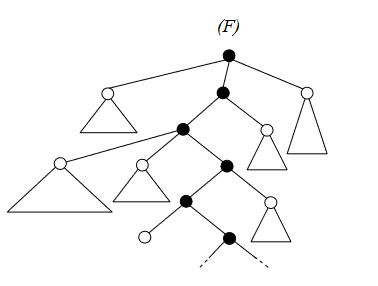
\includegraphics[width=0.6\linewidth]{toplight}
	\label{TopLight set} 
	\centering
\end{figure}
\end{frame}


%------------------------------------------------
\subsection{Key Idea}
\begin{frame}
\frametitle{Key Idea(An Optimal Decomposition Algorithm)}
\begin{itemize}
\item For all $v \in TopLight(F)$, Klein's strategy solves $\delta(F(v), G)$ by determining the direction according to F(v), even if $\left\vert F(v) \right\vert < \left\vert G \right\vert$
\item In such case, making decision according to the larger forest can do better.
\end{itemize}
\end{frame}

%------------------------------------------------
\subsection{Algorithm}
\begin{frame}
\frametitle{Algorithm(An Optimal Decomposition Algorithm)}

We compute $\delta(F, G)$ recursively as follows:
\begin{enumerate}[(1)]
\item if $\left\vert F \right\vert < \left\vert G \right\vert$, compute $\delta(G, F)$ instead.
\item Recursively compute $\delta(F(v), G)$ for all $v \in TopLight(F)$.
\item Compute $\delta(F. G)$ using the following decomposition strategy:
\begin{itemize}
\item S(F', G')=left, if F' is a tree, or the root of leftmost tree is not the heavy child of its parent.
\item Otherwise, S(F', G')=right.
\end{itemize}
\end{enumerate}

\end{frame}

%------------------------------------------------
\subsection{Time Complexity}
\begin{frame}
\frametitle{Time Complexity(An Optimal Decomposition Algorithm)}
\begin{block}{Prerequisite of the Analysis}
\begin{itemize}
\item $\sum_{v \in TopLight(F)}\left\vert F(v) \right\vert \leq \left\vert F \right\vert$.
\item $\left\vert F(v) \right\vert < \frac{\left\vert F \right\vert}{2}$ for each $v \in TopLight(F)$. Otherwise v would be a heavy node.
\item This algorithm consists of two main steps(step 2 and 3). Then algorithm is bounded by $\mathcal{O}(\mathcal{O}(Step2) + \mathcal{O}(Step3))$
\item In step 3, a node v in the heavy path of F cannot be matched or deleted until the remaining subforest is a tree. That is to say only $\left\vert F \right\vert$ subforest need to be considered. This gives $\mathcal{O}(\left\vert F \right\vert \left\vert G \right\vert^ 2)$
\item In step2, the complexity is bound by the number of subforest $\sum_{v \in TopLight(G)}R(F(v), G)$
\end{itemize}

\end{block}
\end{frame}

%------------------------------------------------
\begin{frame}
\frametitle{Time Complexity(An Optimal Decomposition Algorithm)}
\begin{block}{Analysis}
We have established that if $\left\vert F \right\vert \geq \left\vert G \right\vert$
\begin{displaymath}
R(F, G) \leq \left\vert G \right\vert^2 \left\vert F \right\vert + \sum_{v \in TopLight(F)}R(F(v), G)
\end{displaymath}
Otherwise
\begin{displaymath}
R(F, G) \leq \left\vert F \right\vert^2 \left\vert G \right\vert + \sum_{w \in TopLight(G)}R(F, G(w))
\end{displaymath}
\end{block}
\end{frame}

%------------------------------------------------
\begin{frame}
\frametitle{Time Complexity(An Optimal Decomposition Algorithm)}
\begin{block}{Analysis}
\textbf{LEMMA 17} 
\begin{displaymath}
R(F, G) \leq 4(\left\vert F \right\vert \left\vert G \right\vert)^{\frac{3}{2}}
\end{displaymath}
\emph{Proof.}
By applying the induction hypothesis on $R(F(v), G)$
\begin{eqnarray*}
\begin{split}
R(F, G) & \leq \left\vert G \right\vert^2 \left\vert F \right\vert + \sum_{v \in TopLight(F)}4(\left\vert F(v) \right\vert \left\vert G \right\vert)^{\frac{3}{2}}\\
& = \left\vert G \right\vert^2 \left\vert F \right\vert + 4 \left\vert G \right\vert^{\frac{3}{2}}\sum_{v \in TopLight(F)}\left\vert F(v)\right\vert^{\frac{3}{2}}\\
& \leq \left\vert G \right\vert^2 \left\vert F \right\vert + 4 \left\vert G \right\vert^{\frac{3}{2}}\sum_{v \in TopLight(F)}\left\vert F(v)\right\vert max_{v \in TopLight(F)}\sqrt{\left\vert F(v) \right\vert}\\
& \leq \left\vert G \right\vert^2 \left\vert F \right\vert + 4 \left\vert G \right\vert^{\frac{3}{2}}\left\vert F \right\vert \sqrt{\frac{\left\vert F \right\vert}{2}} = \left\vert G \right\vert^2 \left\vert F \right\vert + \sqrt{8}(\left\vert F \right\vert \left\vert G \right\vert)^{\frac{3}{2}} \\
& \leq 4(\left\vert F \right\vert \left\vert G \right\vert)^{\frac{3}{2}}\\
\end{split}
\end{eqnarray*}


\end{block}
\end{frame}

%------------------------------------------------
\section{Optimal Decomposition Strategy}
\begin{frame}
\frametitle{Algorithm}
\begin{block}{For tree-tree edit distance}
\begin{align*}
&\delta(l(f), l'(f')) = min \begin{cases}
	  \delta(f , l'(f')) + \gamma(l \to \lambda) \\ %& \text{deletion of l,}\\
      \delta(l(f), f') + \gamma(\lambda \to l') \\ %& \text{insertion of l',}\\
     \delta(f, f') + \gamma(l \to l') & \\ %\text{replacement of l by l'}
      \end{cases} &
\end{align*}
\end{block}
\begin{block}{For forest-forest edit distance}
\begin{align*}
&\delta(l(f) \comp t, l'(f') \comp t') = min \begin{cases}
	  \delta(f \comp t , l'(f') \comp t') + \gamma(l \to \lambda) \\ %& \text{deletion of l,}\\
      \delta(l(f) \comp t, f' \comp t') + \gamma(\lambda \to l') \\ %& \text{insertion of l',}\\
     \delta(l(f), l'(f')) + \delta(t, t') & \\ %\text{replacement of l by l'}
      \end{cases} &
\end{align*}
\end{block}
\end{frame}


%------------------------------------------------
\begin{frame}
\frametitle{Decomposition Example}
\begin{figure}
	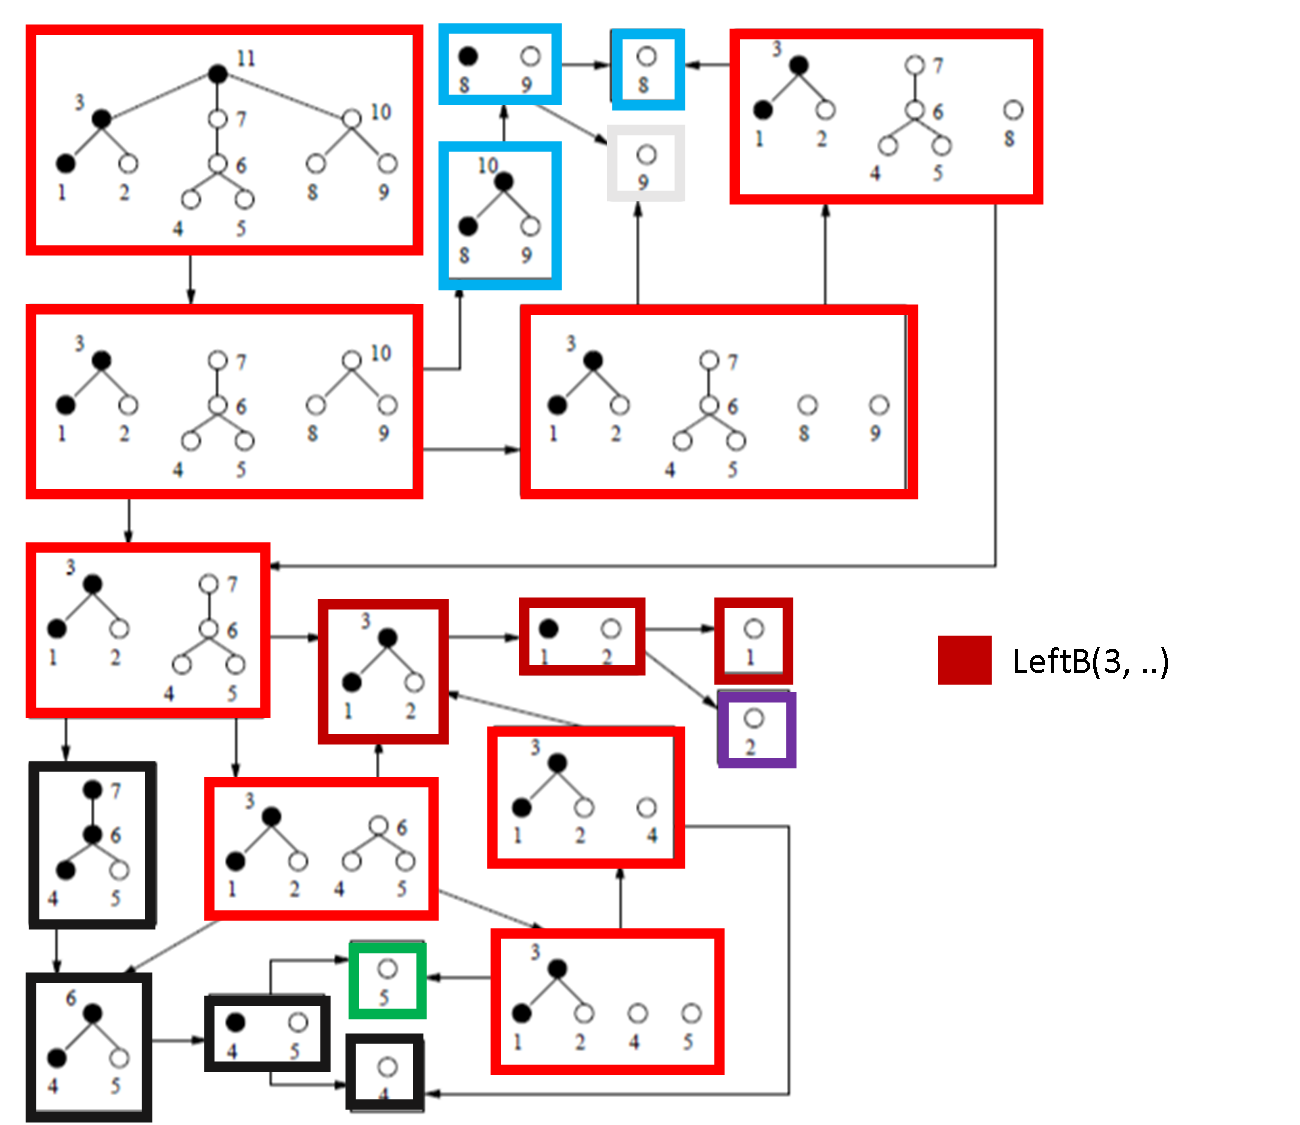
\includegraphics[width=0.7\linewidth]{DecompositionExample}
	\label{Decomposition Example} 
	\centering
\end{figure}
\end{frame}

%------------------------------------------------
\begin{frame}
\frametitle{Definition}
\begin{itemize}
\item \textbf{Free} : the number of sub-problems of tree A compared with tree B.
\item \textbf{LeftA} : the number of sub-problems created by \textbf{right} deletions of tree B(favorite child is the \textbf{leftmost} root of tree B), which are compared with all \textbf{leftmost} forest of tree A.
\item \textbf{RightA} : the number of sub-problems created by \textbf{left} deletions of tree B(favorite child is the \textbf{rightmost} root of tree B), which are compared with all \textbf{rightmost} forest of tree A.
\item \textbf{AllA} : the number of sub-problems after a series of left and right deletions of tree B(favorite child is neither rightmost nor leftmost root of tree B), which are compared with all \textbf{special} forest of tree A. 
\end{itemize}

\textbf{Note}
\begin{itemize}
\item The definitions of \textbf{LeftB}, \textbf{RightB}, \textbf{AllA} are analogy with \textbf{LeftA}, \textbf{RightB}, \textbf{AllA}.
\item The size of each matrix is $\left\vert A \right\vert * \left\vert B \right\vert$.
\end{itemize}
\end{frame}

%------------------------------------------------
\begin{frame}
\frametitle{Number of Rightmost, Leftmost and Subforest.}
Let A be a tree of size n,
\begin{align*}
\#right(A) &= \sum(\left\vert A(i) \right\vert, i \in A) - \sum(\left\vert A(j) \right\vert, j\ is\ a\ rightmost\ child) \\
\#left(A) &= \sum(\left\vert A(i) \right\vert, i \in A) - \sum(\left\vert A(j) \right\vert, j\ is\ a\ leftmost\ child) \\
\#special(A) &= \frac{n(n+3)}{2} - \sum_{i \in A} \left\vert A(i) \right\vert \\
\end{align*}
\textbf{Time Complexity}

To compute the number of rightmost, leftmost and special forests for each subtree whose each root is a node in tree A and tree B. This can be made in $\mathcal{O}(\left\vert A \right\vert + \left\vert B \right\vert)$
\end{frame}

%------------------------------------------------
\begin{frame}
\frametitle{Computation of Free}
\begin{figure}
	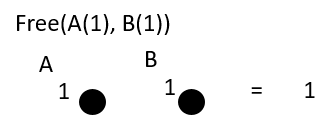
\includegraphics[width=0.4\linewidth]{Free_1_1}
	\label{Free_1_1} 
	\centering
\end{figure}
\begin{figure}
	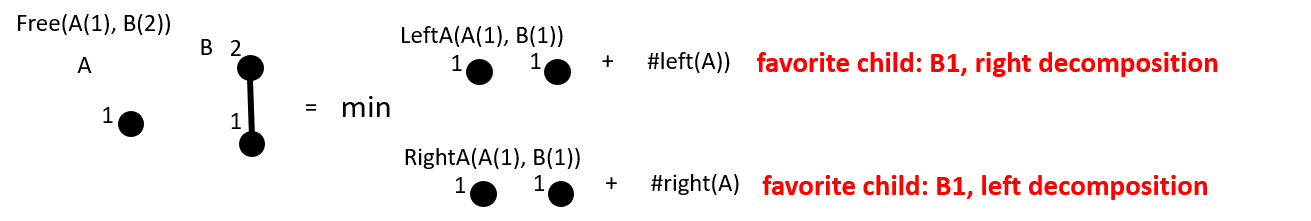
\includegraphics[width=1.1\linewidth]{Free_1_2}
	\label{Free_1_2} 
	\centering
\end{figure}

\end{frame}


%------------------------------------------------
\begin{frame}
\frametitle{Computation of Free}
\begin{figure}
	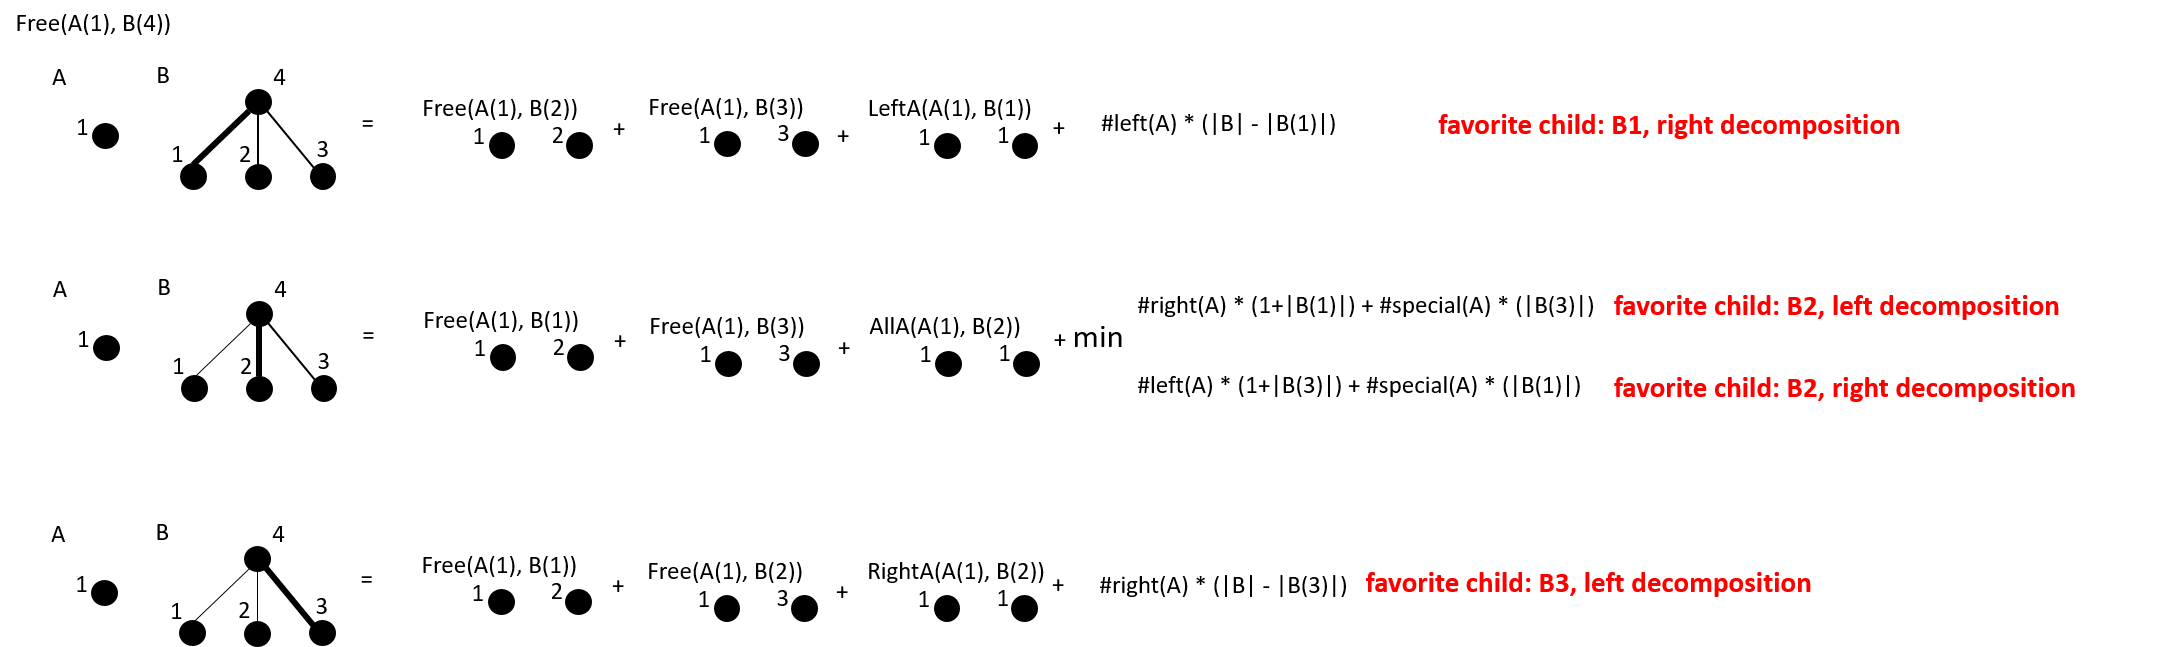
\includegraphics[width=1.0\linewidth]{Free_1_4}
	\label{Free_1_4} 
	\centering
\end{figure}

\end{frame}

%------------------------------------------------
\begin{frame}
\frametitle{Computation of Free}
\begin{figure}
	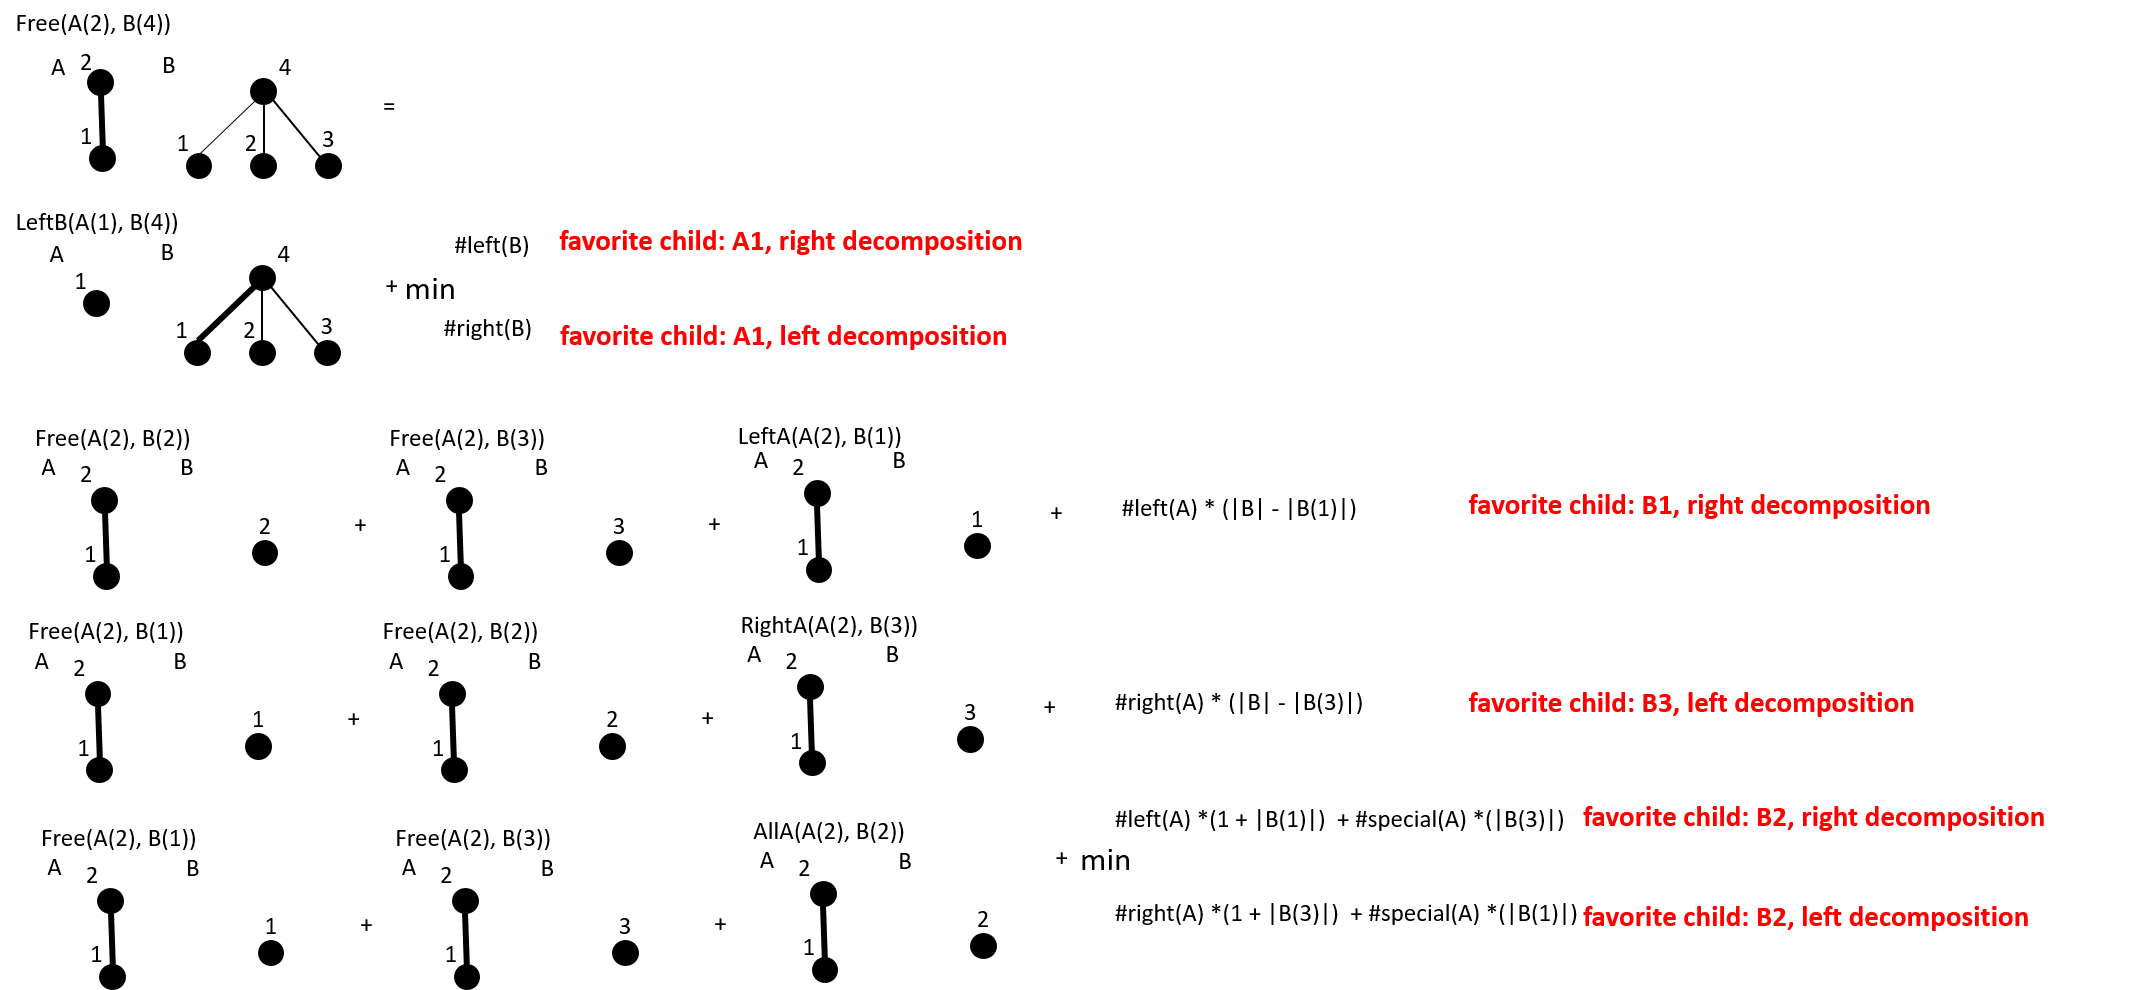
\includegraphics[width=1.0\linewidth]{Free_2_4}
	\label{Free_2_4} 
	\centering
\end{figure}

\end{frame}

%------------------------------------------------
\begin{frame}
\frametitle{Computation of Free}
\begin{figure}
	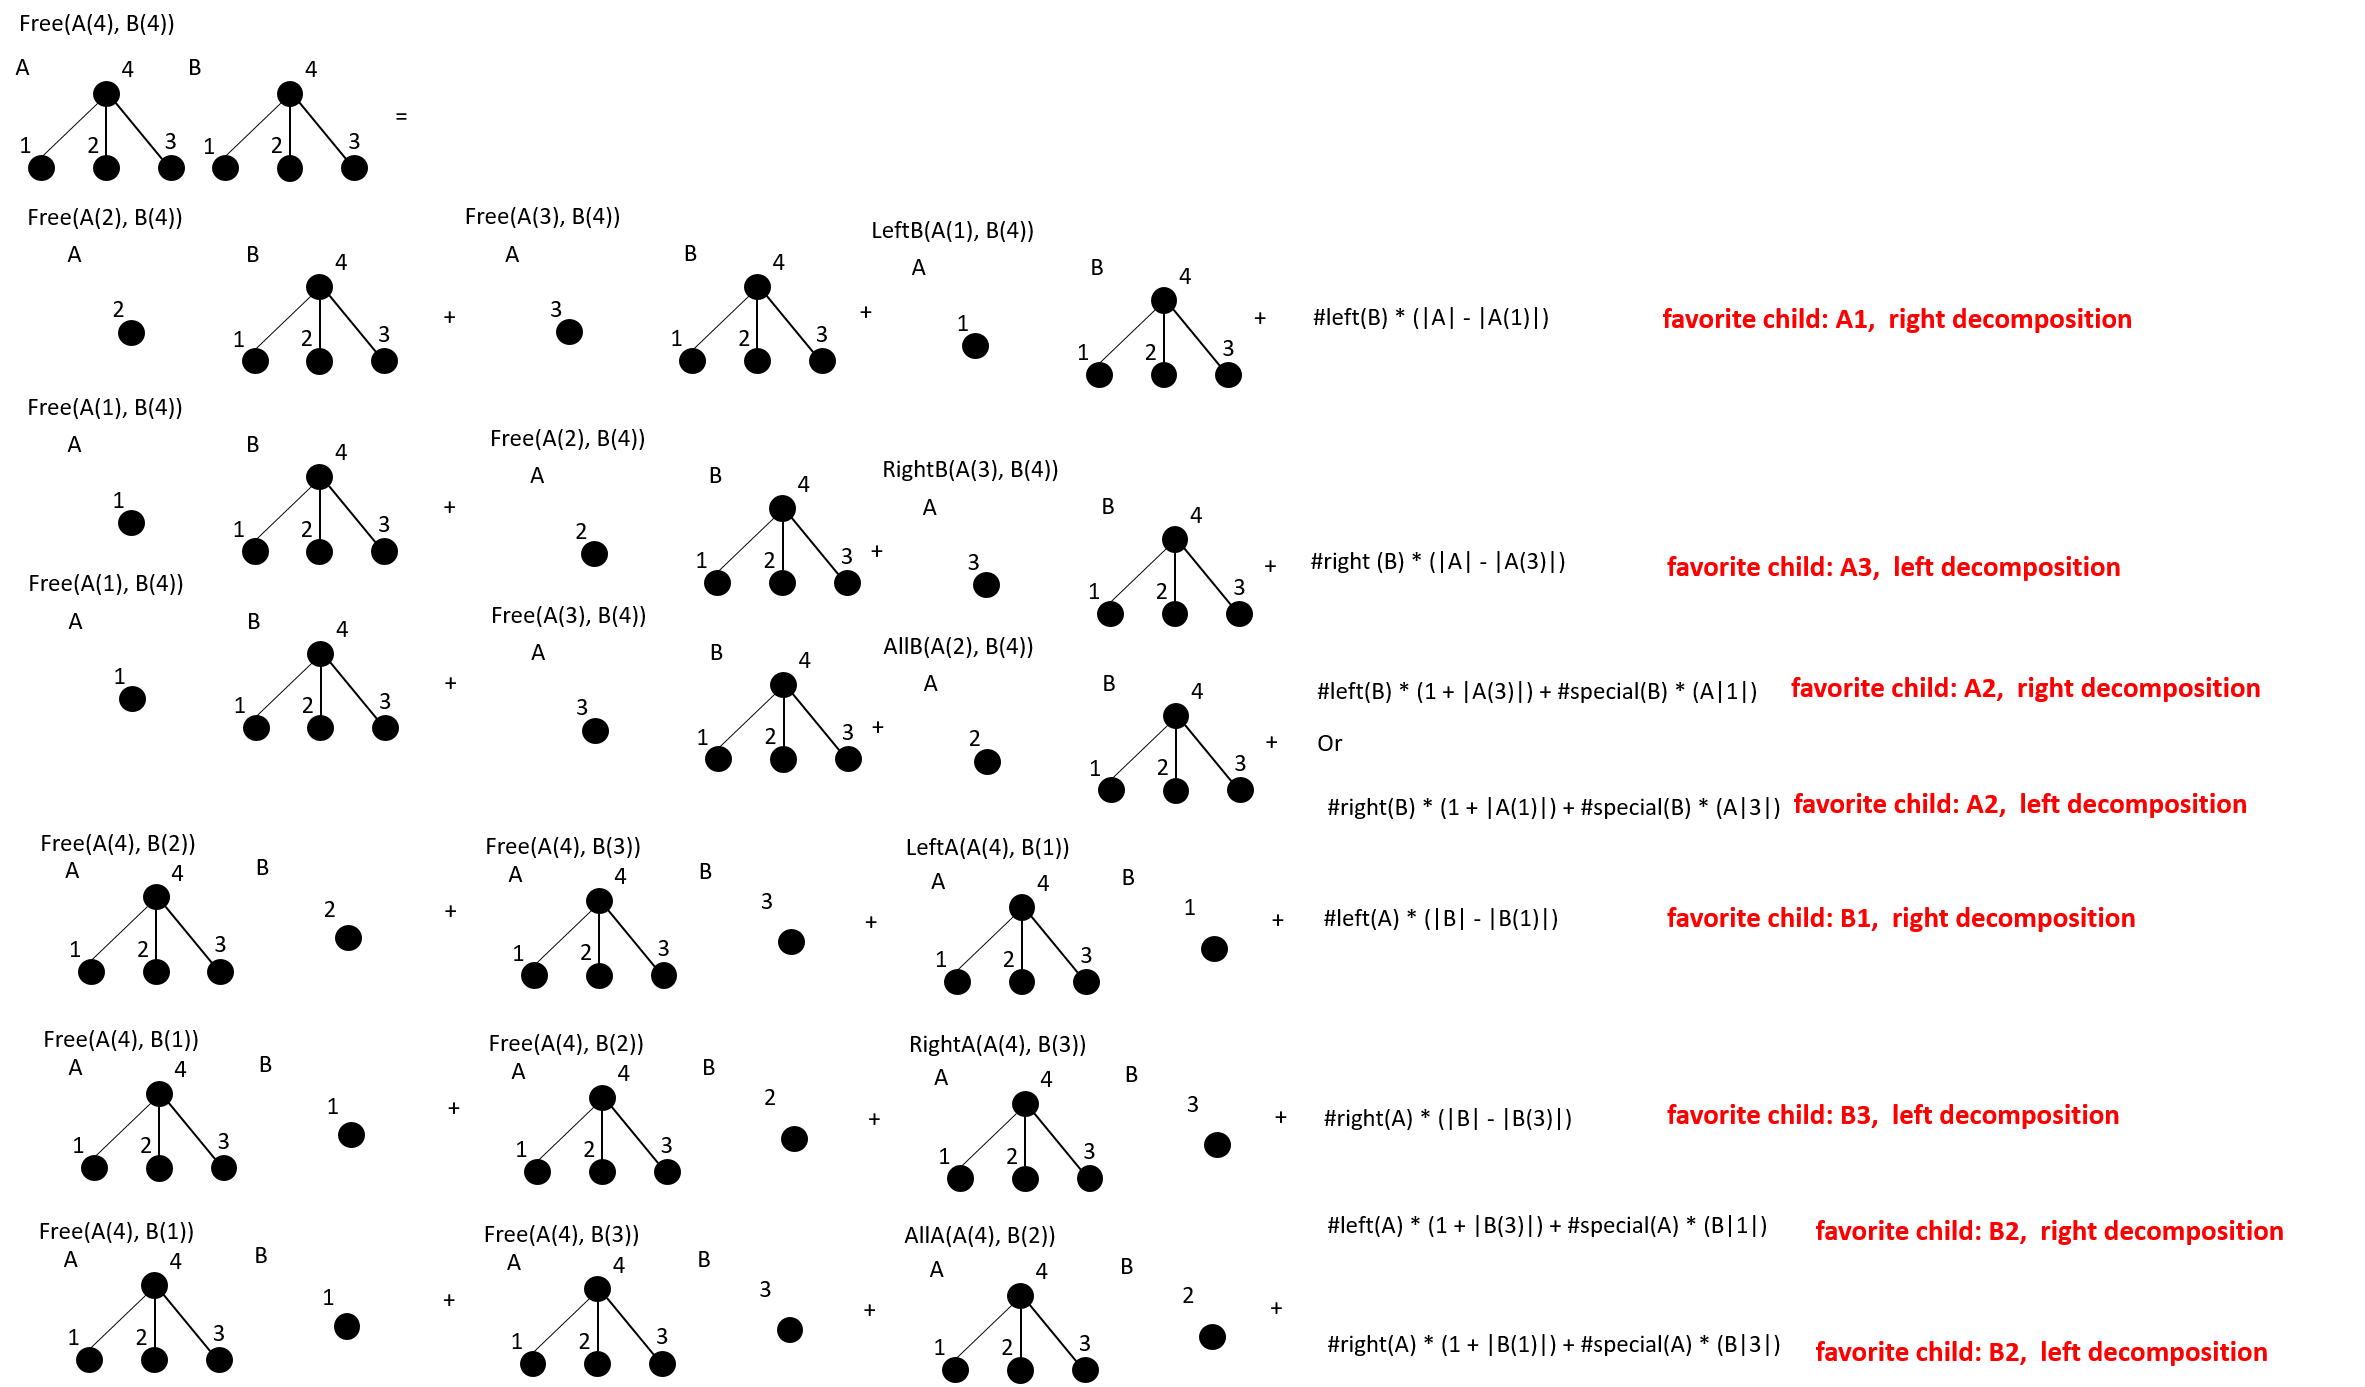
\includegraphics[width=1.0\linewidth]{Free_4_4}
	\label{Free_4_4} 
	\centering
\end{figure}

\end{frame}

%------------------------------------------------
\begin{frame}
\frametitle{Computation of RightA}
\begin{figure}
	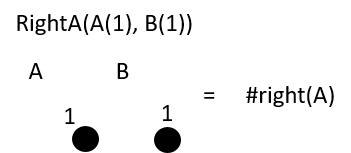
\includegraphics[width=0.4\linewidth]{RightA_1_1}
	\label{RightA_1_1} 
	\centering
\end{figure}
\begin{figure}
	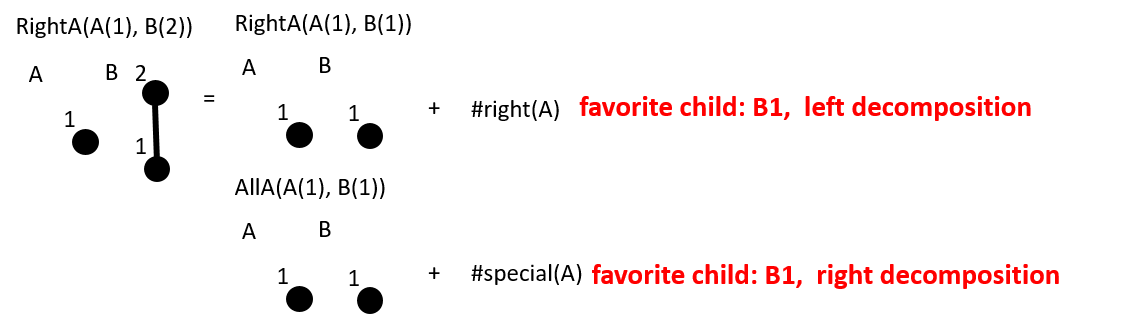
\includegraphics[width=1.1\linewidth]{RightA_1_2}
	\label{RightA_1_2} 
	\centering
\end{figure}

\end{frame}

%------------------------------------------------
\begin{frame}
\frametitle{Computation of RightA}
\begin{figure}
	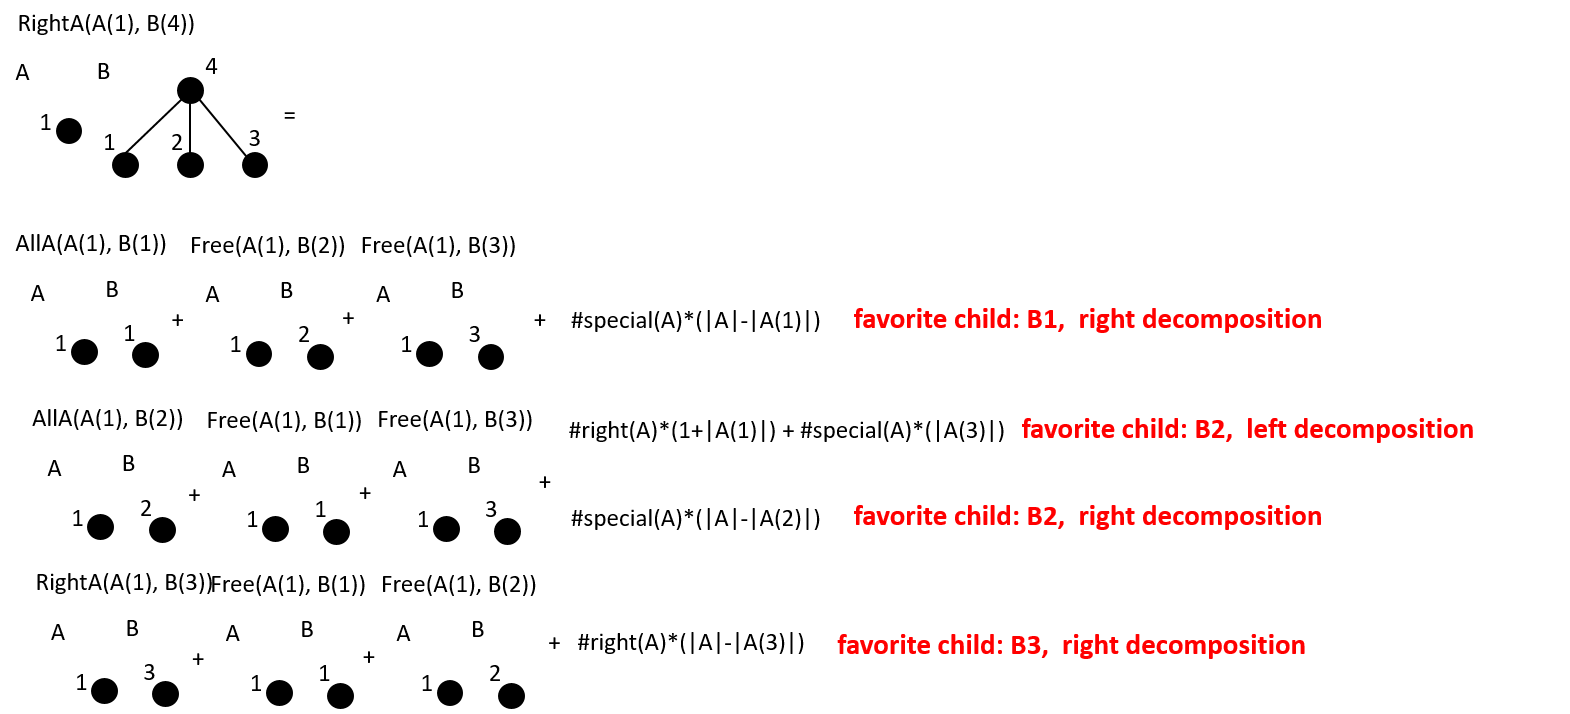
\includegraphics[width=1.0\linewidth]{RightA_1_4}
	\label{RightA_1_4} 
	\centering
\end{figure}

\end{frame}

%------------------------------------------------
\begin{frame}
\frametitle{Computation of RightA}
\begin{figure}
	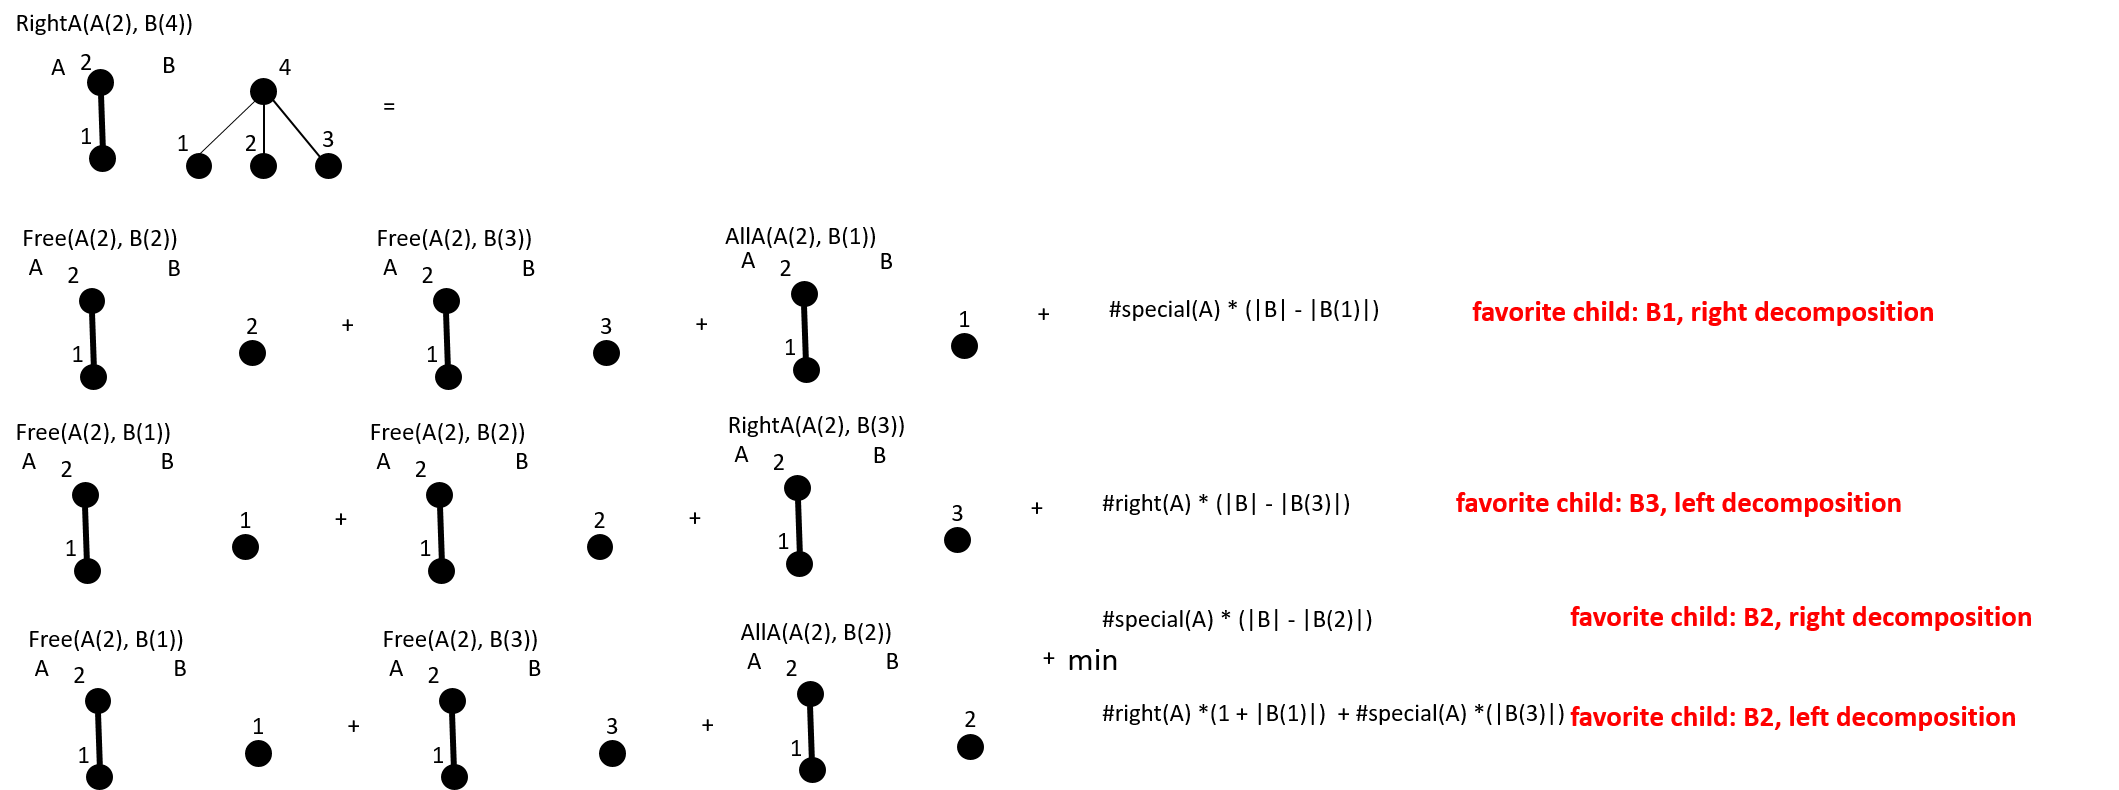
\includegraphics[width=1.0\linewidth]{RightA_2_4}
	\label{RightA_2_4} 
	\centering
\end{figure}

\end{frame}

%------------------------------------------------
\begin{frame}
\frametitle{Computation of RightA}
\begin{figure}
	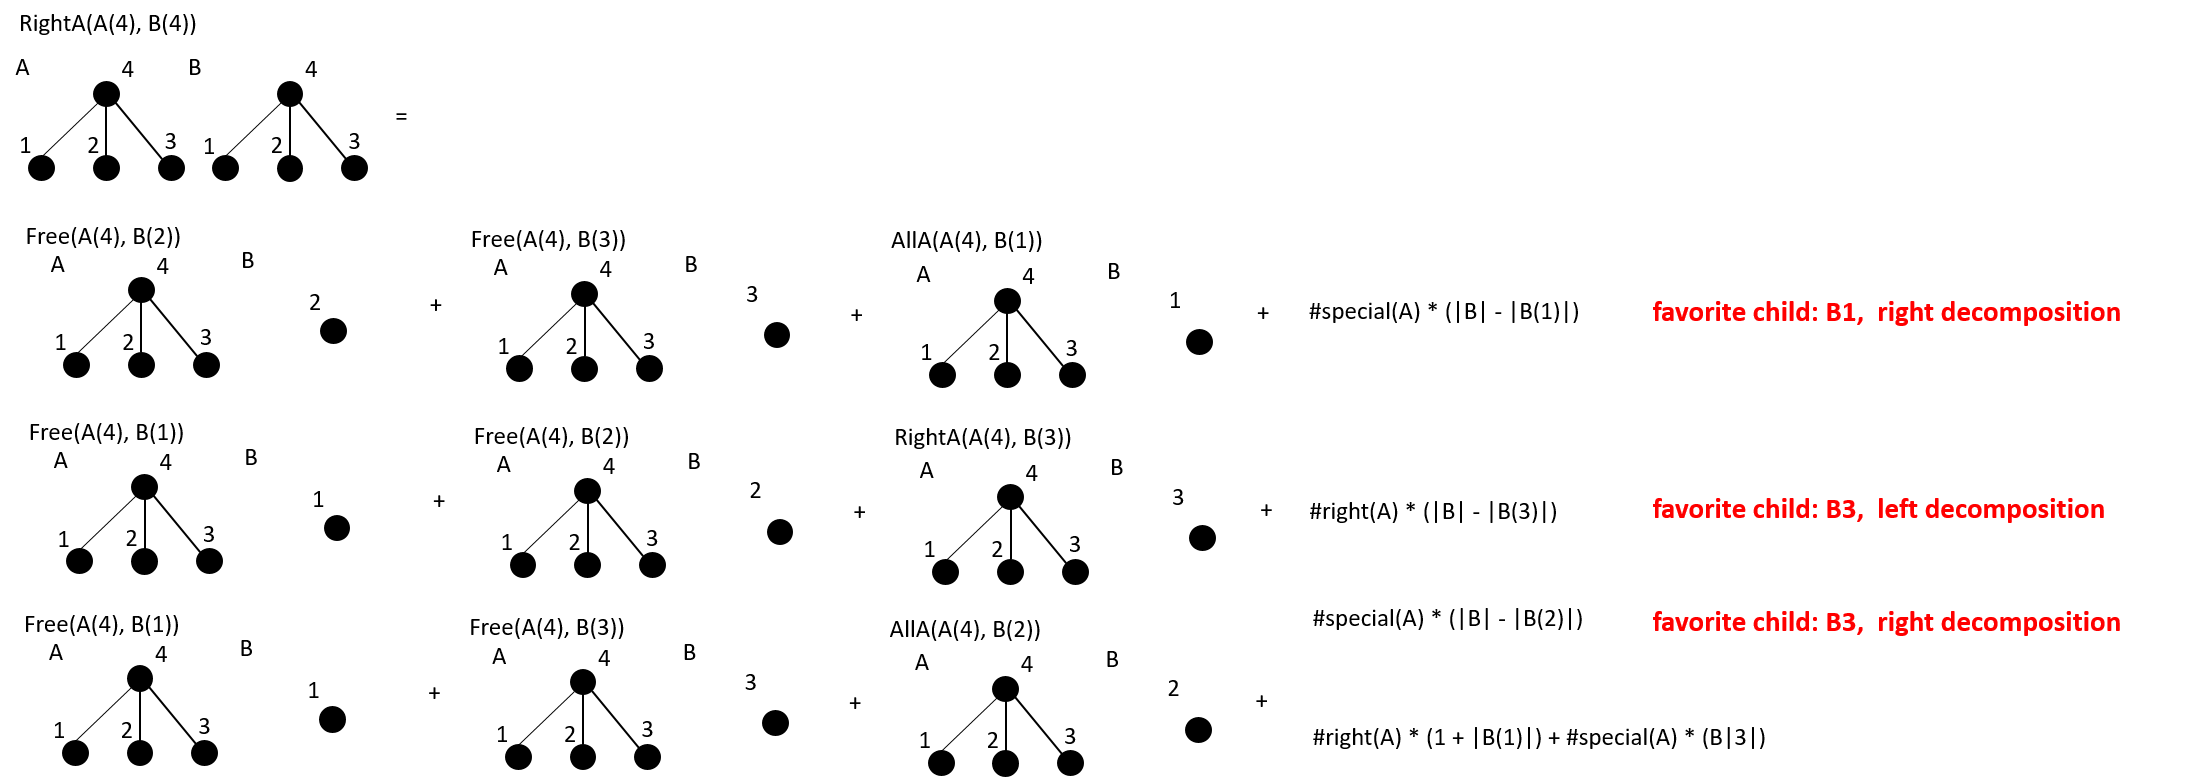
\includegraphics[width=1.0\linewidth]{RightA_4_4}
	\label{RightA_4_4} 
	\centering
\end{figure}

\end{frame}

%------------------------------------------------
\begin{frame}
\frametitle{Computation of RightA}
\begin{figure}
	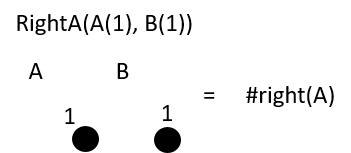
\includegraphics[width=0.4\linewidth]{RightA_1_1}
	\label{RightA_1_1} 
	\centering
\end{figure}
\begin{figure}
	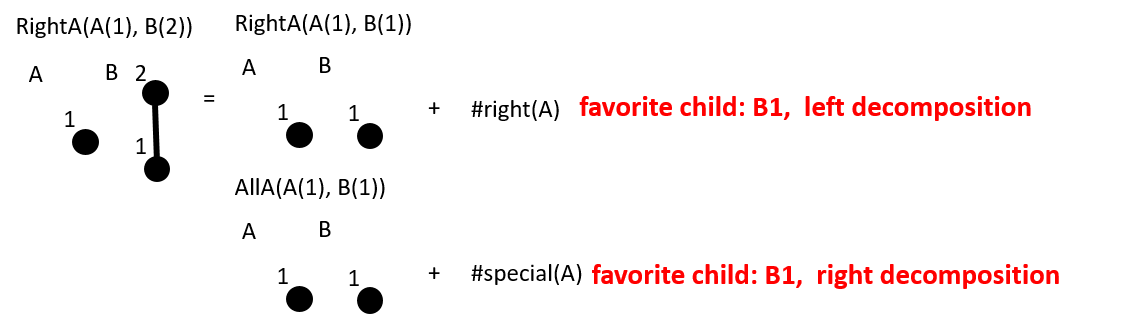
\includegraphics[width=1.1\linewidth]{RightA_1_2}
	\label{RightA_1_2} 
	\centering
\end{figure}

\end{frame}

%------------------------------------------------
\begin{frame}
\frametitle{Computation of RightA}
\begin{figure}
	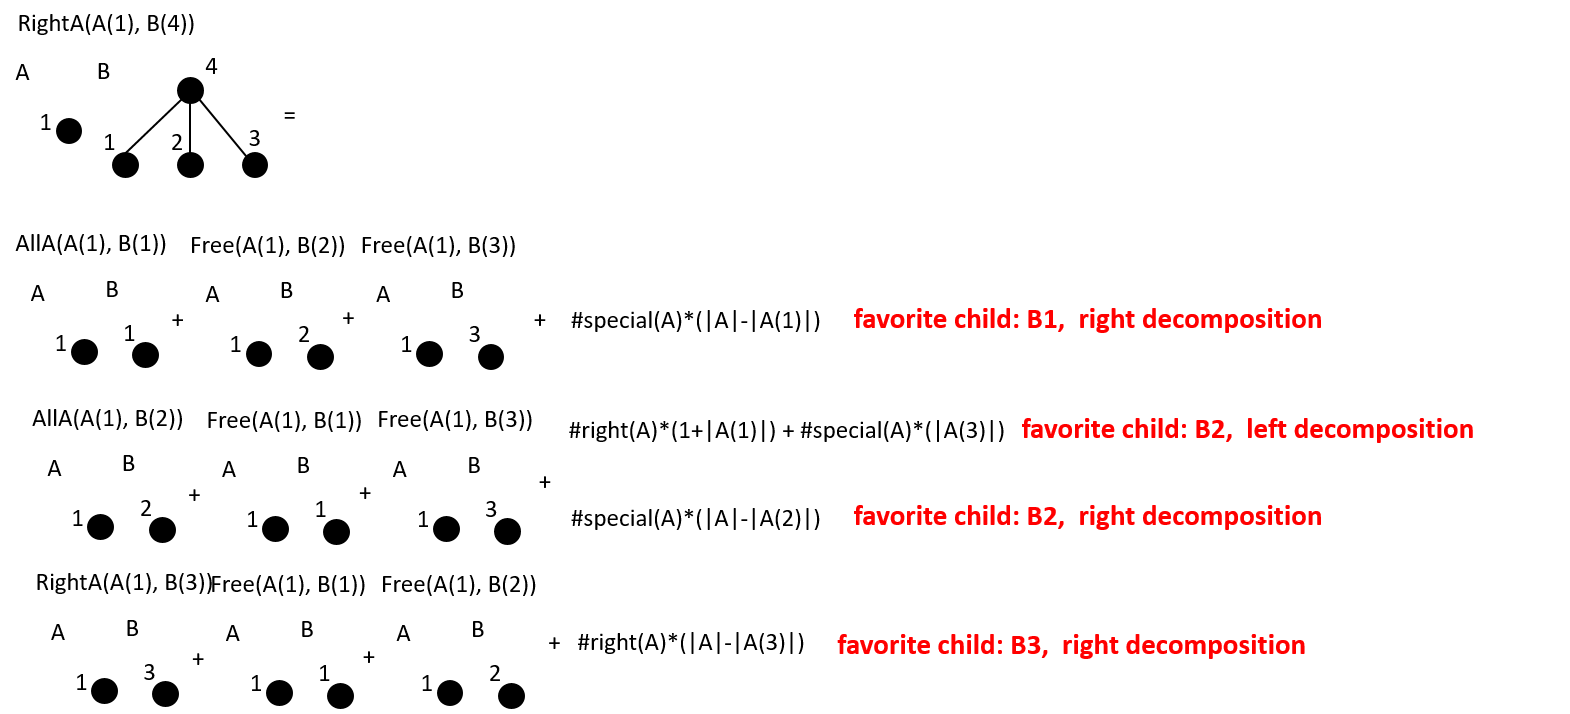
\includegraphics[width=1.0\linewidth]{RightA_1_4}
	\label{RightA_1_4} 
	\centering
\end{figure}

\end{frame}

%------------------------------------------------
\begin{frame}
\frametitle{Computation of RightA}
\begin{figure}
	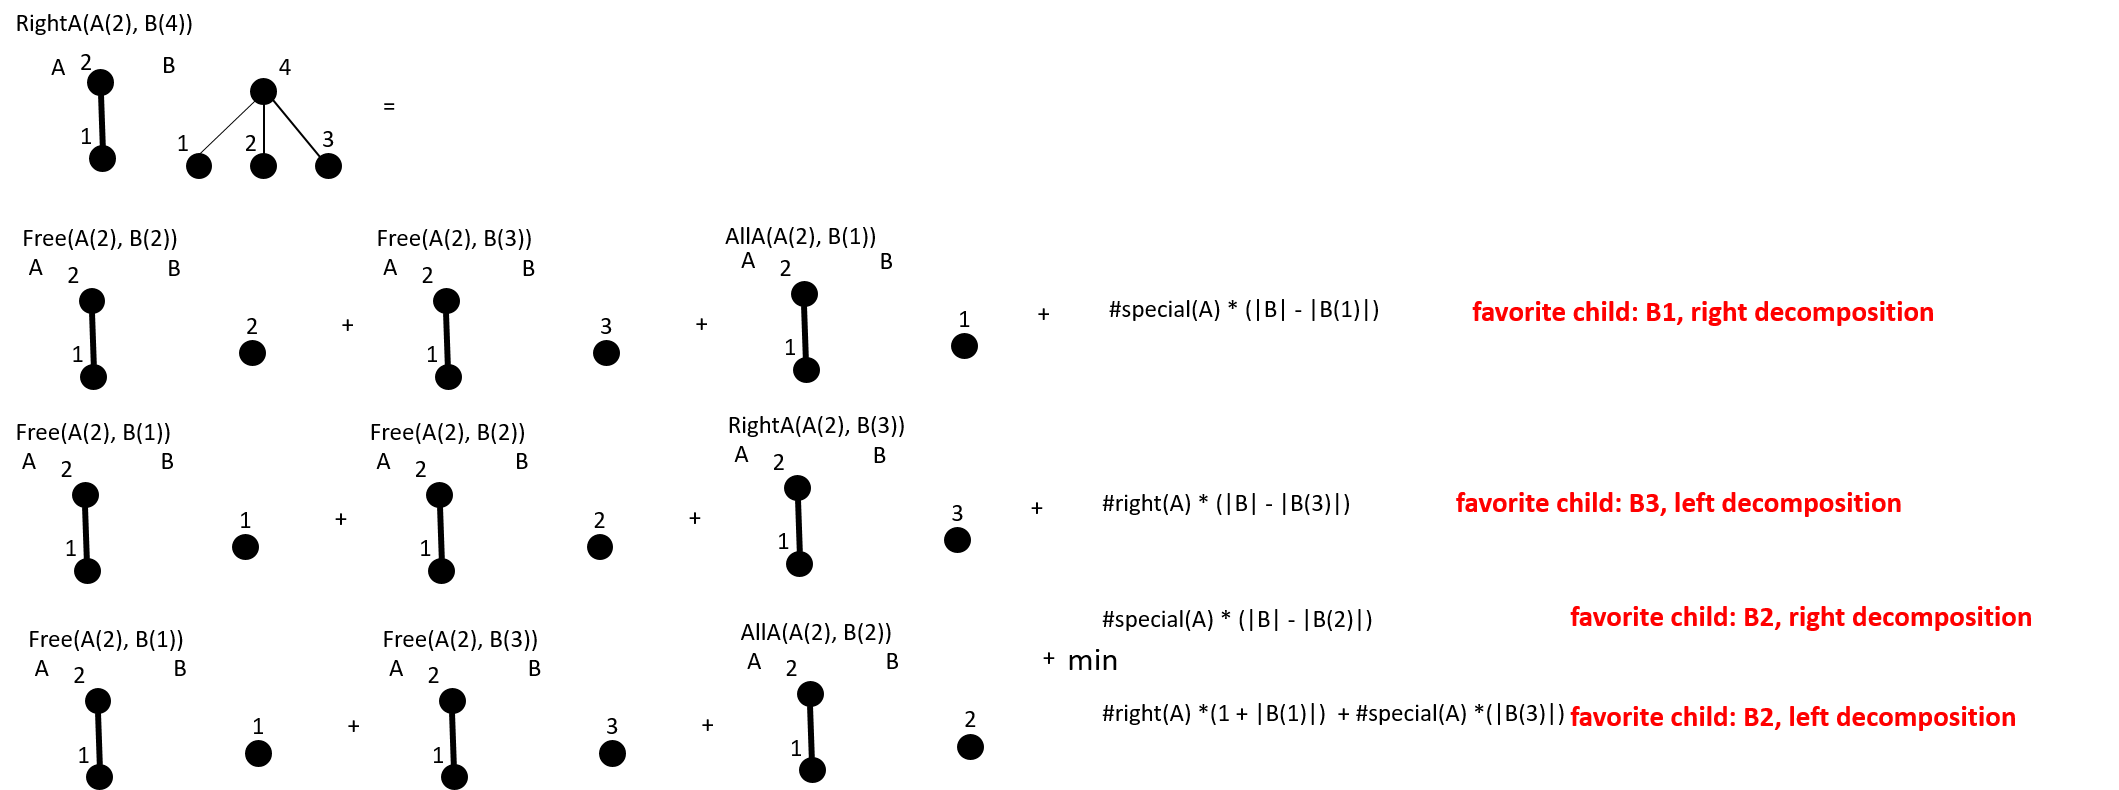
\includegraphics[width=1.0\linewidth]{RightA_2_4}
	\label{RightA_2_4} 
	\centering
\end{figure}

\end{frame}

%------------------------------------------------
\begin{frame}
\frametitle{Computation of RightA}
\begin{figure}
	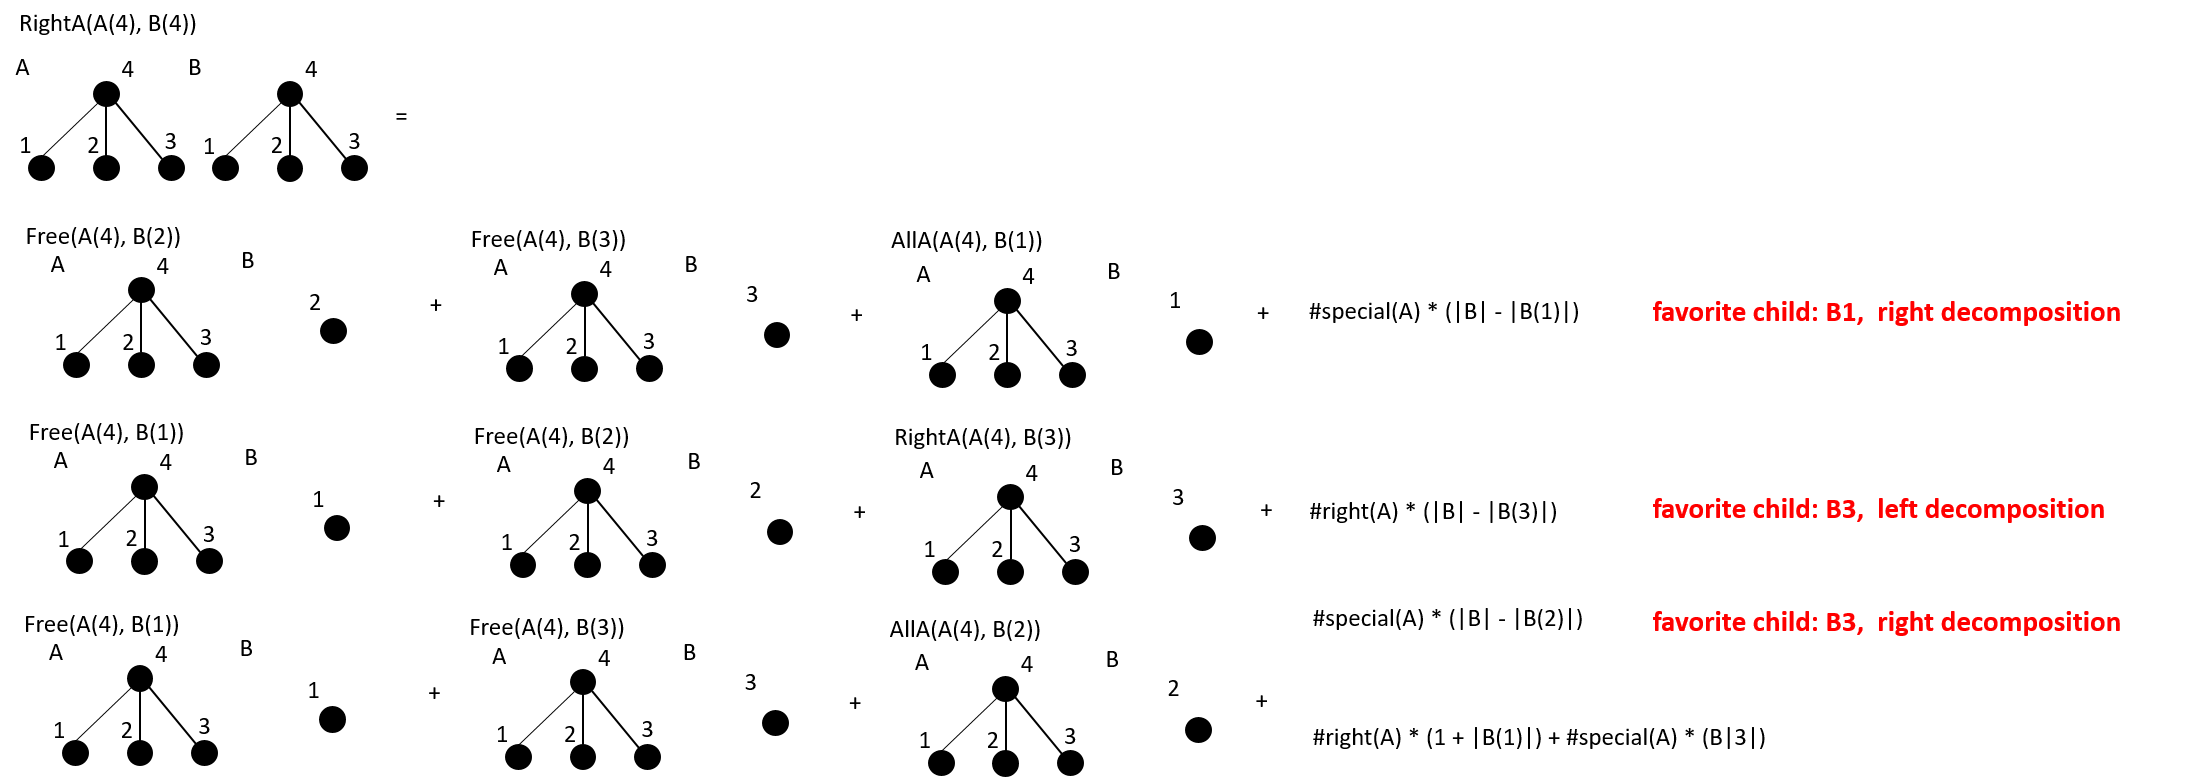
\includegraphics[width=1.0\linewidth]{RightA_4_4}
	\label{RightA_4_4} 
	\centering
\end{figure}

\end{frame}

%------------------------------------------------
\section{Implement}
\begin{frame}
\frametitle{Tree Indexing}
\begin{itemize}
\item $preOrder\_left\_to\_right\ \to\ preL\ $
\item $preOrder\_right\_to\_left\ \to\ preR\ $
\item $postOrder\_left\_to\_right\ \to\ postL\ $
\item $postOrder\_right\_to\_left\ \to\ postR\ $
\end{itemize}
\textbf{Note:}
\begin{itemize}
\item $preL + postR + 1 = treeSize$
\item $preR + postL + 1 = treeSize$
\end{itemize}
\end{frame}
%------------------------------------------------
\begin{frame}
\frametitle{Tree Indexing}
A sequence \textbf{"(B(C(D)(E))(F(G)))"} can be built to a tree F.

Consider a tree F(preL, preR, postL, postR)

\begingroup

\centering
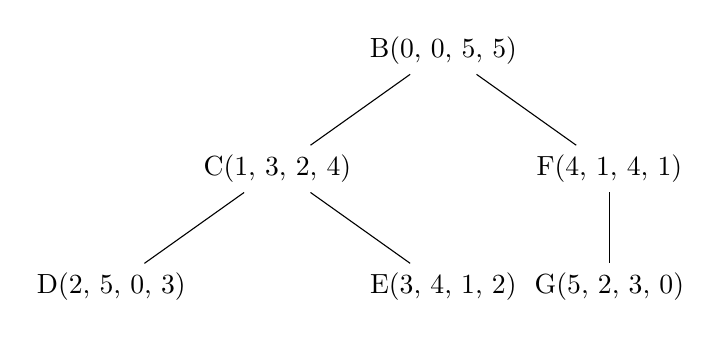
\begin{tikzpicture}[sibling distance=12em]
  \node {B(0, 0, 5, 5)}
    child {node {C(1, 3, 2, 4)}
    	child{node {D(2, 5, 0, 3)}}
    	child{node {E(3, 4, 1, 2)}}
    }
    child {node {F(4, 1, 4, 1)}
      child {node {G(5, 2, 3, 0)}}
    };
\end{tikzpicture}

\endgroup

\textbf{Note:}
\begin{itemize}
\item $preOrder\_left\_to\_right\ \to\ preL\ \to lF$
\item $preOrder\_right\_to\_left\ \to\ preR\ \to rF$
\end{itemize}

\end{frame}

%------------------------------------------------
\begin{frame}
\frametitle{Tree Indexing}
\begin{figure}
	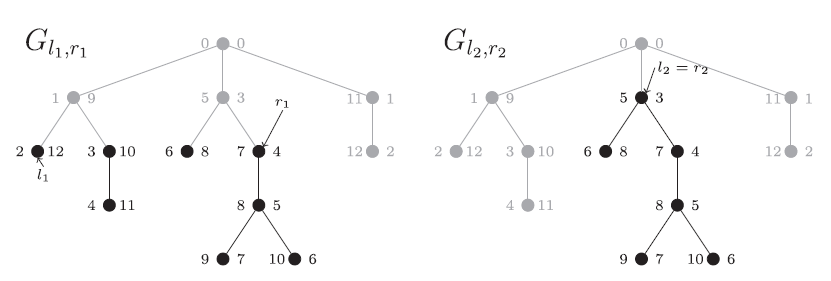
\includegraphics[width=1.0\linewidth]{TreeIndexing}
	\label{TreeIndexing} 
	\centering
\end{figure}
\textbf{Definition:}

$F_{lF, rF}$ is the subforest of F with nodes N($F_{lF, rF}$) = \{$lF$, $rF$\} $\cup$ \{x:x $\in$ F, x succeeds $lF$ in left-to-right preorder and x succeed $rF$ in right-to-left preorder\} and edges E($F_{lF, rF}$) = \{(v, w) $\in$ E(F): v $\in$ $F_{lF, rF} \cap w \in F_{lF, rF}$\}

\end{frame}

%------------------------------------------------
\begin{frame}
\frametitle{Computation of Rightmost, Leftmost and Special Forest}
Let A be a tree of size n,

\begingroup

\centering
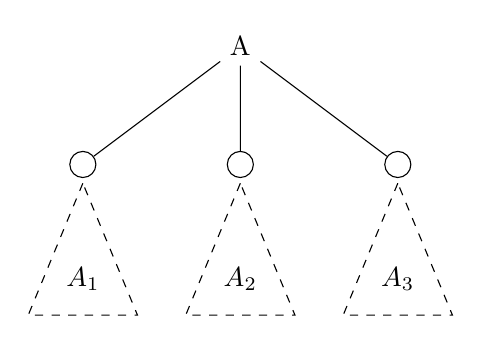
\begin{tikzpicture}
  \tikzstyle{level 1}=[sibling distance=20mm]
  \tikzstyle{level 2}=[sibling distance=5mm]
  \node {A}
    child {node[circle,draw] {}
    	   node[itria] {$A_1$}}
    child {node[circle,draw] {}
    	   node[itria] {$A_2$}} 
    child {node[circle,draw] {}
    	   node[itria] {$A_3$}};
  \centering
\end{tikzpicture}

\endgroup
\begin{align*}
\#right(l(A_1,\cdots, A_n)) &= \sum\#right(A_i) + \left\vert A \right\vert - \left\vert A_n \right\vert \\
\#left(l(A_1,\cdots, A_n)) &= \sum\#left(A_i) + \left\vert A \right\vert - \left\vert A_1 \right\vert \\
\#special(A) &= \frac{n(n+3)}{2} - \sum_{i \in A} \left\vert A(i) \right\vert \\
\end{align*}

\end{frame}

%------------------------------------------------
\begin{frame}
\frametitle{Computation of Rightmost, Leftmost and Special Forest}
Let A be a tree of size n,

\begin{align*}
\#right(l(A_1,\cdots, A_n)) &= \sum\#right(A_i) + \left\vert A \right\vert - \left\vert A_n \right\vert \\
\#left(l(A_1,\cdots, A_n)) &= \sum\#left(A_i) + \left\vert A \right\vert - \left\vert A_1 \right\vert \\
\#special(A) &= \frac{n(n+3)}{2} - \sum_{i \in A} \left\vert A(i) \right\vert \\
\end{align*}

\textbf{Note:}
Each node marks
\begin{itemize}
\item the size of subtree rooted at that node
\item the sum of the size of subtree of its chilren
\item the number of leftmost forest of subtree rooted at that node
\item the number of rightmost forest of subtree rooted at that node
\item the number of special forest of subtree rooted at that node
\end{itemize} 

\end{frame}

%------------------------------------------------
\begin{frame}
\frametitle{Special Forest Enumeration}
Let G be a tree,
\begingroup

\centering
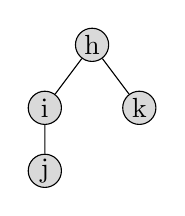
\begin{tikzpicture}[level distance=8mm]
  \tikzstyle{level 1}=[sibling distance=12mm]
  \tikzstyle{level 2}=[sibling distance=5mm]
  \node[vertex] {h}
    child {node[vertex] {i}
    	child {node[vertex] {j}}
    	  }
  	child {node[vertex] {k}};
\end{tikzpicture}

\endgroup

Then the \textbf{left-to-right} enumeration would be 
\begin{itemize}
\item lG = k


\begin{tikzpicture}[level distance=8mm]
  \tikzstyle{level 1}=[sibling distance=12mm]
  \tikzstyle{level 2}=[sibling distance=5mm]
  \node[vertex] {k};
\end{tikzpicture}
(rG = k)

\item lG = j


\begin{tikzpicture}[level distance=8mm]
  \tikzstyle{level 1}=[sibling distance=12mm]
  \tikzstyle{level 2}=[sibling distance=5mm]
  \node[vertex] {j};
\end{tikzpicture}
(rG = j)\hspace{1cm}

\begin{tikzpicture}[level distance=8mm]
  \tikzstyle{level 1}=[sibling distance=12mm]
  \tikzstyle{level 2}=[sibling distance=5mm]
  \node[vertex] {j};
\end{tikzpicture}

\begin{tikzpicture}[level distance=8mm]
  \tikzstyle{level 1}=[sibling distance=12mm]
  \tikzstyle{level 2}=[sibling distance=5mm]
  \node[vertex] {k};
\end{tikzpicture}
(rG = k)

\item lG = i


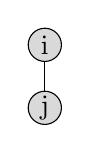
\begin{tikzpicture}[level distance=8mm]
  \tikzstyle{level 1}=[sibling distance=12mm]
  \tikzstyle{level 2}=[sibling distance=5mm]
  \node[vertex] {i}
  	child{ node[vertex] {j}};
\end{tikzpicture}
(rG = i)\hspace{1cm}
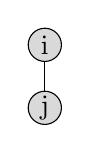
\begin{tikzpicture}[level distance=8mm]
  \tikzstyle{level 1}=[sibling distance=12mm]
  \tikzstyle{level 2}=[sibling distance=5mm]
  \node[vertex] {i}
  	child{ node[vertex] {j}};
\end{tikzpicture}

\begin{tikzpicture}[level distance=8mm]
  \tikzstyle{level 1}=[sibling distance=12mm]
  \tikzstyle{level 2}=[sibling distance=5mm]
  \node[vertex] {k};
\end{tikzpicture}
(rG = k)

\end{itemize}
\end{frame}

%------------------------------------------------
\begin{frame}
\frametitle{Special Forest Enumeration}
Let G be a tree,
\begingroup

\centering
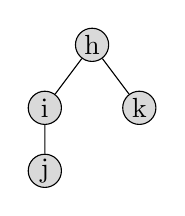
\begin{tikzpicture}[level distance=8mm]
  \tikzstyle{level 1}=[sibling distance=12mm]
  \tikzstyle{level 2}=[sibling distance=5mm]
  \node[vertex] {h}
    child {node[vertex] {i}
    	child {node[vertex] {j}}
    	  }
  	child {node[vertex] {k}};
\end{tikzpicture}

\endgroup
\begin{itemize}
\item lG = h

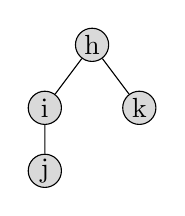
\begin{tikzpicture}[level distance=8mm]
  \tikzstyle{level 1}=[sibling distance=12mm]
  \tikzstyle{level 2}=[sibling distance=5mm]
  \node[vertex] {h}
    child {node[vertex] {i}
    	child {node[vertex] {j}}
    	  }
  	child {node[vertex] {k}};
\end{tikzpicture}
(rG = h)\hspace{1cm}


\end{itemize}
\end{frame}

%------------------------------------------------
\begin{frame}
\frametitle{Special Forest Enumeration}
Let G be a tree,
\begingroup

\centering
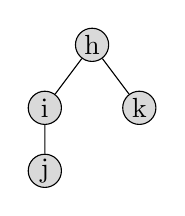
\begin{tikzpicture}[level distance=8mm]
  \tikzstyle{level 1}=[sibling distance=12mm]
  \tikzstyle{level 2}=[sibling distance=5mm]
  \node[vertex] {h}
    child {node[vertex] {i}
    	child {node[vertex] {j}}
    	  }
  	child {node[vertex] {k}};
\end{tikzpicture}

\endgroup

Then the \textbf{right-to-left} enumeration would be 
\begin{itemize}
\item rG = j


\begin{tikzpicture}[level distance=8mm]
  \tikzstyle{level 1}=[sibling distance=12mm]
  \tikzstyle{level 2}=[sibling distance=5mm]
  \node[vertex] {j};
\end{tikzpicture}
(lG = j)

\item rG = i

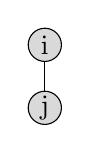
\begin{tikzpicture}[level distance=8mm]
  \tikzstyle{level 1}=[sibling distance=12mm]
  \tikzstyle{level 2}=[sibling distance=5mm]
  \node[vertex] {i}
  	child{ node[vertex] {j}};
\end{tikzpicture}
(lG = i)\hspace{1cm}

\item rG = k


\begin{tikzpicture}[level distance=8mm]
  \tikzstyle{level 1}=[sibling distance=12mm]
  \tikzstyle{level 2}=[sibling distance=5mm]
  \node[vertex] {k};
\end{tikzpicture}
(lG = k)\hspace{1cm}

\begin{tikzpicture}[level distance=8mm]
  \tikzstyle{level 1}=[sibling distance=12mm]
  \tikzstyle{level 2}=[sibling distance=5mm]
  \node[vertex] {j};
\end{tikzpicture}

\begin{tikzpicture}[level distance=8mm]
  \tikzstyle{level 1}=[sibling distance=12mm]
  \tikzstyle{level 2}=[sibling distance=5mm]
  \node[vertex] {k};
\end{tikzpicture}
(lG = j)\hspace{1cm}
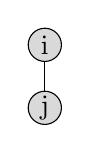
\begin{tikzpicture}[level distance=8mm]
  \tikzstyle{level 1}=[sibling distance=12mm]
  \tikzstyle{level 2}=[sibling distance=5mm]
  \node[vertex] {i}
  	child{ node[vertex] {j}};
\end{tikzpicture}

\begin{tikzpicture}[level distance=8mm]
  \tikzstyle{level 1}=[sibling distance=12mm]
  \tikzstyle{level 2}=[sibling distance=5mm]
  \node[vertex] {k};
\end{tikzpicture}
(lG = i)

\end{itemize}
\end{frame}

%------------------------------------------------
\begin{frame}
\frametitle{Special Forest Enumeration}
Let G be a tree,
\begingroup

\centering
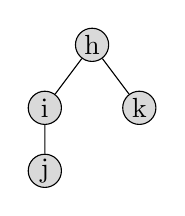
\begin{tikzpicture}[level distance=8mm]
  \tikzstyle{level 1}=[sibling distance=12mm]
  \tikzstyle{level 2}=[sibling distance=5mm]
  \node[vertex] {h}
    child {node[vertex] {i}
    	child {node[vertex] {j}}
    	  }
  	child {node[vertex] {k}};
\end{tikzpicture}

\endgroup
\begin{itemize}
\item rG = h

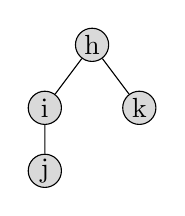
\begin{tikzpicture}[level distance=8mm]
  \tikzstyle{level 1}=[sibling distance=12mm]
  \tikzstyle{level 2}=[sibling distance=5mm]
  \node[vertex] {h}
    child {node[vertex] {i}
    	child {node[vertex] {j}}
    	  }
  	child {node[vertex] {k}};
\end{tikzpicture}
(lG = h)


\end{itemize}
\end{frame}

%------------------------------------------------
\begin{frame}
\frametitle{Special Forest Enumeration}
Let G be a tree,

\hspace{3cm}
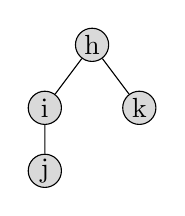
\begin{tikzpicture}[level distance=8mm]
  \tikzstyle{level 1}=[sibling distance=12mm]
  \tikzstyle{level 2}=[sibling distance=5mm]
  \node[vertex] {h}
    child {node[vertex] {i}
    	child {node[vertex] {j}}
    	  }
  	child {node[vertex] {k}};
\end{tikzpicture}\hspace{3cm}
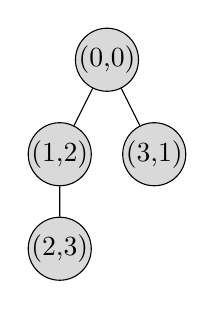
\begin{tikzpicture}[level distance=12mm]
  \tikzstyle{level 1}=[sibling distance=12mm]
  \tikzstyle{level 2}=[sibling distance=5mm]
  \node[vertex] {(0,0)}
    child {node[vertex] {(1,2)}
    	child {node[vertex] {(2,3)}}
    	  }
  	child {node[vertex] {(3,1)}};
\end{tikzpicture}


\begin{itemize}
\item left-to-right
\begin{itemize}
\item lG enumerate in reverse left to right pre-order.
\item rG enumerate from subset right(G, lG) $\cup$ lG in reverse right to left pre-order.
\end{itemize} 
\item right-to-left
\begin{itemize}
\item rG enumerate in reverse right to left pre-order.
\item lG enumerate from subset left(G, rG) $\cup$ rG in reverse left to right pre-order
\end{itemize}
\end{itemize}
\end{frame}

%------------------------------------------------
\begin{frame}
\frametitle{Rightmost Forest Enumeration - right path decomposition}
Let G be a tree,
\begingroup

\centering
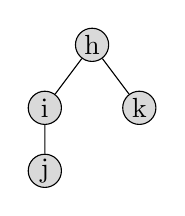
\begin{tikzpicture}[level distance=8mm]
  \tikzstyle{level 1}=[sibling distance=12mm]
  \tikzstyle{level 2}=[sibling distance=5mm]
  \node[vertex] {h}
    child {node[vertex] {i}
    	child {node[vertex] {j}}
    	  }
  	child {node[vertex] {k}};
\end{tikzpicture}

\endgroup
\begin{itemize}
\item rG = j


\begin{tikzpicture}[level distance=8mm]
  \tikzstyle{level 1}=[sibling distance=12mm]
  \tikzstyle{level 2}=[sibling distance=5mm]
  \node[vertex] {j};
\end{tikzpicture}
(lG = j)
\item rG = i

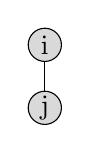
\begin{tikzpicture}[level distance=8mm]
  \tikzstyle{level 1}=[sibling distance=12mm]
  \tikzstyle{level 2}=[sibling distance=5mm]
  \node[vertex] {i}
  	child {node[vertex] {j}};
\end{tikzpicture}
(lG = i)
\item rG = k


\begin{tikzpicture}[level distance=8mm]
  \tikzstyle{level 1}=[sibling distance=12mm]
  \tikzstyle{level 2}=[sibling distance=5mm]
  \node[vertex] {k};
\end{tikzpicture}
(lG = k)\hspace{1cm}

\begin{tikzpicture}[level distance=8mm]
  \tikzstyle{level 1}=[sibling distance=12mm]
  \tikzstyle{level 2}=[sibling distance=5mm]
  \node[vertex] {j};
\end{tikzpicture}

\begin{tikzpicture}[level distance=8mm]
  \tikzstyle{level 1}=[sibling distance=12mm]
  \tikzstyle{level 2}=[sibling distance=5mm]
  \node[vertex] {k};
\end{tikzpicture}
(lG = j)\hspace{1cm}
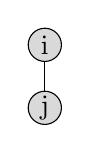
\begin{tikzpicture}[level distance=8mm]
  \tikzstyle{level 1}=[sibling distance=12mm]
  \tikzstyle{level 2}=[sibling distance=5mm]
  \node[vertex] {i}
  	child {node[vertex] {j}};
\end{tikzpicture}

\begin{tikzpicture}[level distance=8mm]
  \tikzstyle{level 1}=[sibling distance=12mm]
  \tikzstyle{level 2}=[sibling distance=5mm]
  \node[vertex] {k};
\end{tikzpicture}
(lG = i)

\end{itemize}
\end{frame}

%------------------------------------------------
\begin{frame}
\frametitle{Rightmost Forest Enumeration - right path decomposition}
Let G be a tree,
\begingroup

\centering
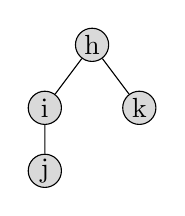
\begin{tikzpicture}[level distance=8mm]
  \tikzstyle{level 1}=[sibling distance=12mm]
  \tikzstyle{level 2}=[sibling distance=5mm]
  \node[vertex] {h}
    child {node[vertex] {i}
    	child {node[vertex] {j}}
    	  }
  	child {node[vertex] {k}};
\end{tikzpicture}

\endgroup
\begin{itemize}
\item lG = h

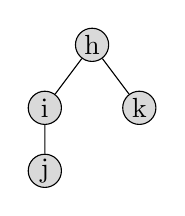
\begin{tikzpicture}[level distance=8mm]
  \tikzstyle{level 1}=[sibling distance=12mm]
  \tikzstyle{level 2}=[sibling distance=5mm]
  \node[vertex] {h}
    child {node[vertex] {i}
    	child {node[vertex] {j}}
    	  }
  	child {node[vertex] {k}};
\end{tikzpicture}
(rG = h)
\end{itemize}
\end{frame}

%------------------------------------------------
\begin{frame}
\frametitle{Leftmost Forest Enumeration - left path decomposition}
Let G be a tree,
\begingroup

\centering
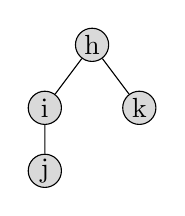
\begin{tikzpicture}[level distance=8mm]
  \tikzstyle{level 1}=[sibling distance=12mm]
  \tikzstyle{level 2}=[sibling distance=5mm]
  \node[vertex] {h}
    child {node[vertex] {i}
    	child {node[vertex] {j}}
    	  }
  	child {node[vertex] {k}};
\end{tikzpicture}

\endgroup
\begin{itemize}

\item lG = k


\begin{tikzpicture}[level distance=8mm]
  \tikzstyle{level 1}=[sibling distance=12mm]
  \tikzstyle{level 2}=[sibling distance=5mm]
  \node[vertex] {j};
\end{tikzpicture}
(rG = k)
\item lG = j


\begin{tikzpicture}[level distance=8mm]
  \tikzstyle{level 1}=[sibling distance=12mm]
  \tikzstyle{level 2}=[sibling distance=5mm]
  \node[vertex] {j};
\end{tikzpicture}
(rG = j)
\item lG = i

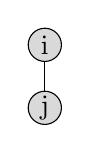
\begin{tikzpicture}[level distance=8mm]
  \tikzstyle{level 1}=[sibling distance=12mm]
  \tikzstyle{level 2}=[sibling distance=5mm]
  \node[vertex] {i}
  	child {node[vertex] {j}};
\end{tikzpicture}
(rG = i)\hspace{1cm}
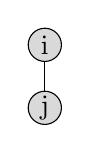
\begin{tikzpicture}[level distance=8mm]
  \tikzstyle{level 1}=[sibling distance=12mm]
  \tikzstyle{level 2}=[sibling distance=5mm]
  \node[vertex] {i}
  	child {node[vertex] {j}};
\end{tikzpicture}

\begin{tikzpicture}[level distance=8mm]
  \tikzstyle{level 1}=[sibling distance=12mm]
  \tikzstyle{level 2}=[sibling distance=5mm]
  \node[vertex] {k};
\end{tikzpicture}
(rG = k)
\end{itemize}
\end{frame}

%------------------------------------------------
\begin{frame}
\frametitle{Leftmost Forest Enumeration - left path decomposition}
Let G be a tree,
\begingroup

\centering
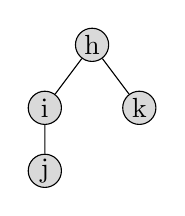
\begin{tikzpicture}[level distance=8mm]
  \tikzstyle{level 1}=[sibling distance=12mm]
  \tikzstyle{level 2}=[sibling distance=5mm]
  \node[vertex] {h}
    child {node[vertex] {i}
    	child {node[vertex] {j}}
    	  }
  	child {node[vertex] {k}};
\end{tikzpicture}

\endgroup
\begin{itemize}
\item rG = h

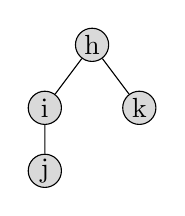
\begin{tikzpicture}[level distance=8mm]
  \tikzstyle{level 1}=[sibling distance=12mm]
  \tikzstyle{level 2}=[sibling distance=5mm]
  \node[vertex] {h}
    child {node[vertex] {i}
    	child {node[vertex] {j}}
    	  }
  	child {node[vertex] {k}};
\end{tikzpicture}
(lG = h)


\end{itemize}
\end{frame}

%------------------------------------------------
\begin{frame}
\frametitle{Leftmost/Rightmost Forest Enumeration}
Let G be a tree,

\hspace{3cm}
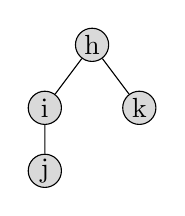
\begin{tikzpicture}[level distance=8mm]
  \tikzstyle{level 1}=[sibling distance=12mm]
  \tikzstyle{level 2}=[sibling distance=5mm]
  \node[vertex] {h}
    child {node[vertex] {i}
    	child {node[vertex] {j}}
    	  }
  	child {node[vertex] {k}};
\end{tikzpicture}\hspace{3cm}
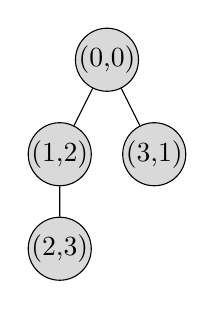
\begin{tikzpicture}[level distance=12mm]
  \tikzstyle{level 1}=[sibling distance=12mm]
  \tikzstyle{level 2}=[sibling distance=5mm]
  \node[vertex] {(0,0)}
    child {node[vertex] {(1,2)}
    	child {node[vertex] {(2,3)}}
    	  }
  	child {node[vertex] {(3,1)}};
\end{tikzpicture}

\begin{itemize}
\item leftmost forest enumeration
\begin{itemize}
\item lG enumerate in reverse left to right pre-order.
\item rG enumerate from subset right(G', lG) $\cup$ lG in reverse right to left pre-order.
\end{itemize}
\item rightmost forest enumeration
\begin{itemize}
\item rG enumerate in reverse right to left pre-order.
\item lG enumerate from subset left(G', lG) $\cup$ lG in reverse left to right pre-order.
\end{itemize}
\end{itemize}
\end{frame}

%------------------------------------------------
\begin{frame}
\frametitle{Leftmost/Rightmost Forest Enumeration}
G' 
\begin{figure}
	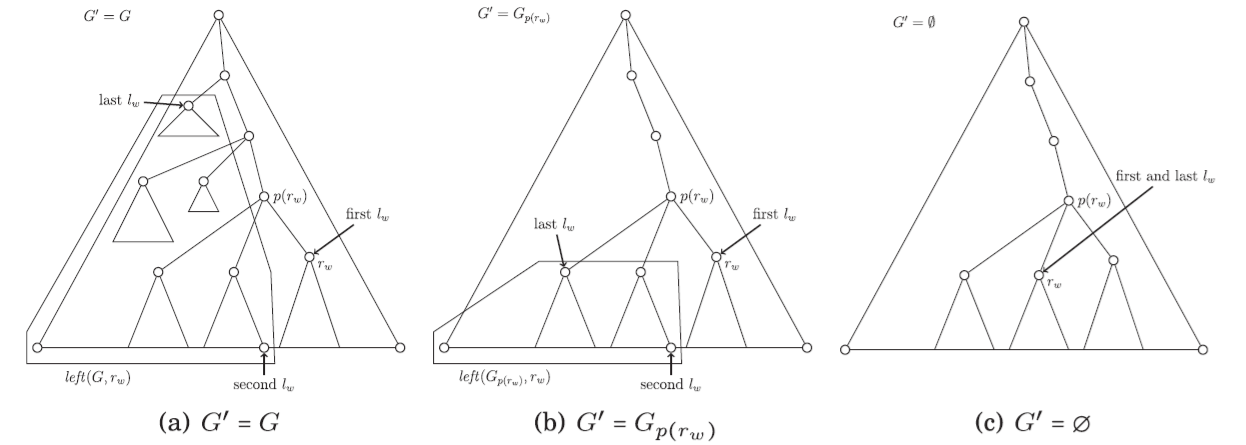
\includegraphics[width=0.9\linewidth]{Dloop}
	\label{Dloop} 
	\centering
\end{figure}
\begin{itemize}
\item special forest enumeration G' = G
\item leftmost forest enumeration
\begin{itemize}
\item lG is the leftmost child of its parent G' = $G_p(lG)$
\item otherwise G'= $\varnothing$
\end{itemize}
\item rightmost forest enumeration
\begin{itemize}
\item rG is the rightmost child of its parent G' = $G_(rG)$
\item otherwise G' = $\varnothing$
\end{itemize}
\end{itemize}

\end{frame}

%------------------------------------------------
\begin{frame}
\frametitle{Leftmost/Rightmost Forest Enumeration}
\begin{columns}[c]
\column{.5\textwidth}
left($F_{p(v)}$, $v$)
\begin{figure}
	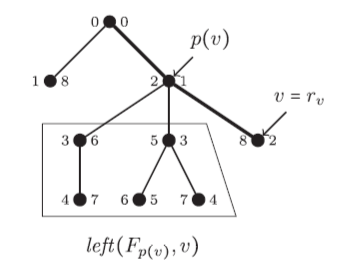
\includegraphics[width=0.8\linewidth]{leftFPV}
	\label{leftFPV} 
	\centering
\end{figure}
\column{.5\textwidth}
left($G$, $w$)
\begin{figure}
	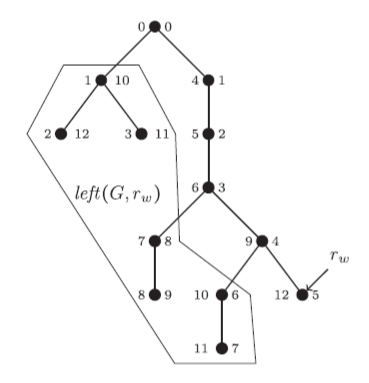
\includegraphics[width=0.8\linewidth]{leftF}
	\label{leftF} 
	\centering
\end{figure}
\end{columns}

\end{frame}
%------------------------------------------------
\begin{frame}
\frametitle{Sub Problem Enumeration}
Enumerate quadruples(lF, rF, lG, rG) in loops (A(BCD)(B'C'D)).
\begin{itemize}
\item Loop A is the outermost loop and iterates bottom-up over the nodes of path.
\begin{figure}
	\includegraphics[width=0.2\linewidth]{Aloop}
	\label{Aloop} 
	\centering
\end{figure}
\item Loop C iterates over the nodes to the left of path γ , in particular, over the nodes
left(Fp(v), v) for a given node v, where v is the index variable of loop A.
\item Loop C' is symmetric to loop C and iterates over the nodes right(Fp(v), v) $\cup$ {p(v)}.
\end{itemize}
\end{frame}

%------------------------------------------------
\begin{frame}
\frametitle{Subproblem Enumeration(Tree F Enumeration)}
\begin{figure}
	\includegraphics[width=0.8\linewidth]{Cloop}
	\label{Cloop} 
	\centering
\end{figure}
\begin{figure}
	\includegraphics[width=0.8\linewidth]{C'loop}
	\label{C'loop} 
	\centering
\end{figure}
\end{frame}

%------------------------------------------------
\begin{frame}
\frametitle{Subproblem Enumeration}
Enumerate quadruples(lF, rF, lG, rG) in loops (A(BCD)(B'C'D)).
\begin{itemize}
\item Loops B and D define subforests of the right-hand tree G.
\end{itemize}
\begin{figure}
	\includegraphics[width=0.2\linewidth]{Bloop}
	\label{Bloop} 
	\centering
\end{figure}
\begin{figure}
	\includegraphics[width=0.8\linewidth]{Dloop}
	\label{Dloop} 
	\centering
\end{figure}
\end{frame}
%------------------------------------------------
\begin{frame}
\frametitle{Efficient Space Complexity}
\begin{itemize}
\item Time complexity in average $\mathcal{O}$($n^3$):
\begin{itemize}
\item The path decomposition in F create n sub forests.
\item The all decomposition in G create $n^2$ sub forests.
\end{itemize}
\item The naive implement leads to the space complexity in average $\mathcal{O}$($n^3$), but can be reduced to $\mathcal{O}$($n^2$)
\end{itemize}

\end{frame}

%------------------------------------------------
\begin{frame}
\frametitle{The intermediate subforest enumeration}
The intermediate subforest enumeration with respect to $F(V_{p-1})$ and $F(V_p)$ is the sequence of forests $F(V_{p-1}) = F_0, F_1 \cdots F_5 = F(V_p)$
\begin{figure}
	\includegraphics[width=0.8\linewidth]{PathDecomposition}
	\label{PathDecomposition} 
	\centering
\end{figure}

\end{frame}

%------------------------------------------------
\begin{frame}
\frametitle{The intermediate subforest enumeration} 
\begin{align*}
&\delta_{L}(F_{lF, rF}, G_{lG, rG}) = min \begin{cases}
	  \delta(F_{lF, rF} - lF , G_{lG, rG}) + \gamma(lF \to \lambda) \\ %& \text{deletion of l,}\\
      \delta(F_{lF, rF}, G_{lG, rG} - lG) + \gamma(\lambda \to lG) \\ %& \text{insertion of l',}\\
     \delta(F_{lF, rF} - F_{lF}, G_{lG, rG} - F_{lG}) 
     \\ \ \ \ + \delta(F_{lF} - lF, G_{lG} - lG) + \gamma(lF \to lG) & \\ %\text{replacement of l by l'}
      \end{cases} &
\end{align*}

\end{frame}

%------------------------------------------------
\begin{frame}
\frametitle{$\mathcal{O}$($n^2$) Space Complexity Implement}
Four Memorization tables: D, S, T, and Q
\begin{itemize}
\item D(of size $\left\vert F\right\vert \left\vert G\right\vert$) stores distance values which are needed across different calls of the single-path function. Subproblems in D are \textbf{pairs of subtrees without their root nodes}.
\item S(of size $\left\vert F\right\vert \left\vert G\right\vert$) stores all subproblems computed in the two innermost loops C(lF in left decompose) and D(lG in left decompose) or C'(rF in right decompose) and D'(rG in right decompose) for specific nodes in the outer loops.$\to$ maintain in each round in B and B'.
\item T(of size $\left\vert G\right\vert^2$) stores distances between \textbf{a specific subforest in F} and \textbf{each relevant subforest of G}. The subforest is either a subtree rooted on the path or a subforest $F_{l'_v, v}$ where $l'_v$ is the leftmost child of p(v).
\item Q(of size $\left\vert F\right\vert$) stores distances between \textbf{each subforest of F defined in loop C}(path decomposition) and \textbf{a specific subforest} in G of the form $G_{p(r_G)-p(r_G)}$, that \textbf{is a subtree in G without root node}. used for the next C loop.
\end{itemize}

\end{frame}

%------------------------------------------------
\begin{frame}
\frametitle{$\mathcal{O}$($n^2$) Space Complexity Implement}
\textbf{Tables indexing:}

For $\delta_L(F_{lF, rF}, G_{lG, rG})$
\begin{itemize}
\item D: $D[preR\_to\_preL(rF), preR\_to\_preL[rG]]$
\item S: $S[lF, lG]$
\item T: $T[lG, rG]$
\item Q: $Q[lF]$ 
\end{itemize}

For $\delta_R(F_{lF, rF}, G_{lG, rG})$
\begin{itemize}
\item D: $D[lF, rF]$
\item S: $S[rF, rG]$
\item T: $T[lG, rG]$
\item Q: $Q[rF]$
\end{itemize}

\end{frame}

%------------------------------------------------
\begin{frame}
\frametitle{$\mathcal{O}$($n^2$) Space Complexity Implement - Example}
Let F and G be two trees

\hspace{3cm}
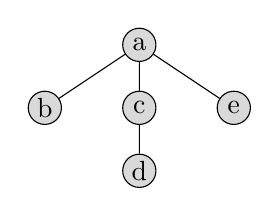
\begin{tikzpicture}[level distance=8mm]
  \tikzstyle{level 1}=[sibling distance=12mm]
  \tikzstyle{level 2}=[sibling distance=5mm]
  \node[vertex] {a}
    child {node[vertex] {b}}
    child {node[vertex] {c}
    	child {node[vertex] {d}}
    	  }
  	child {node[vertex] {e}};
\end{tikzpicture}\hspace{3cm}
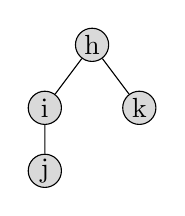
\begin{tikzpicture}[level distance=8mm]
  \tikzstyle{level 1}=[sibling distance=12mm]
  \tikzstyle{level 2}=[sibling distance=5mm]
  \node[vertex] {h}
    child {node[vertex] {i}
    	child {node[vertex] {j}}
    	  }
  	child {node[vertex] {k}};
\end{tikzpicture}

T[
\hspace{3cm}
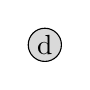
\begin{tikzpicture}[level distance=8mm]
  \tikzstyle{level 1}=[sibling distance=12mm]
  \tikzstyle{level 2}=[sibling distance=5mm]
  \node[vertex] {d};
\end{tikzpicture}\hspace{3cm}

\begin{tikzpicture}[level distance=8mm]
  \tikzstyle{level 1}=[sibling distance=12mm]
  \tikzstyle{level 2}=[sibling distance=5mm]
  \node[vertex] {k};
\end{tikzpicture}

\end{frame}

\end{document} 
